% This file was created (at least in part) by the script ParseMdtoLatex by Louis du Plessis
% (Available from https://github.com/taming-the-beast)

\documentclass[11pt]{article}
\usepackage{amsmath}
\usepackage{amssymb}
%%%%%%%%%%%%%%%%%%%%%%%%%%%%%%%%%%%%%%%%%%%%%%%%%%%%%%%%%%%%%%%
% DO NOT EDIT THIS FILE UNLESS YOU KNOW WHAT YOU ARE DOING!!! %
%%%%%%%%%%%%%%%%%%%%%%%%%%%%%%%%%%%%%%%%%%%%%%%%%%%%%%%%%%%%%%%

% Useful packages
\usepackage[]{authblk}
\usepackage{graphicx}
\usepackage{color}
\usepackage{longtable}
\usepackage{hanging}
\usepackage{indentfirst}
\usepackage{setspace}
\usepackage{enumitem}
\usepackage{verbatim}
\usepackage{upgreek}
\usepackage{framed}
\usepackage{textcomp}
\usepackage{url}
\usepackage{soul}
\usepackage{amsmath,amsfonts,amssymb,mathrsfs}
\usepackage{fancyhdr}
\usepackage[compact]{titlesec}
\usepackage[T1]{fontenc}
\usepackage{lmodern}
\usepackage[utf8]{inputenc}
\usepackage[]{listings}
%\usepackage{fontspec}
\usepackage{placeins}
\usepackage{epstopdf}
\usepackage[export]{adjustbox}
\usepackage{tikz}
\usepackage[breaklinks]{hyperref}
\usepackage[all]{hypcap}


% References
\usepackage[backend=bibtex,hyperref=true,citestyle=authoryear,bibstyle=authortitle,firstinits=true,terseinits=true,doi=false,url=false,eprint=false,maxbibnames=10,maxcitenames=2]{biblatex}
\DeclareCiteCommand{\cite}
  {\usebibmacro{prenote}}
  {\usebibmacro{citeindex}%
   \printtext[bibhyperref]{\usebibmacro{cite}}}
  {\multicitedelim}
  {\usebibmacro{postnote}}

\DeclareCiteCommand*{\cite}
  {\usebibmacro{prenote}}
  {\usebibmacro{citeindex}%
   \printtext[bibhyperref]{\usebibmacro{citeyear}}}
  {\multicitedelim}
  {\usebibmacro{postnote}}

\DeclareCiteCommand{\parencite}[\mkbibparens]
  {\usebibmacro{prenote}}
  {\usebibmacro{citeindex}%
    \printtext[bibhyperref]{\usebibmacro{cite}}}
  {\multicitedelim}
  {\usebibmacro{postnote}}

\DeclareCiteCommand*{\parencite}[\mkbibparens]
  {\usebibmacro{prenote}}
  {\usebibmacro{citeindex}%
    \printtext[bibhyperref]{\usebibmacro{citeyear}}}
  {\multicitedelim}
  {\usebibmacro{postnote}}

\DeclareCiteCommand{\footcite}[\mkbibfootnote]
  {\usebibmacro{prenote}}
  {\usebibmacro{citeindex}%
  \printtext[bibhyperref]{ \usebibmacro{cite}}}
  {\multicitedelim}
  {\usebibmacro{postnote}}

\DeclareCiteCommand{\footcitetext}[\mkbibfootnotetext]
  {\usebibmacro{prenote}}
  {\usebibmacro{citeindex}%
   \printtext[bibhyperref]{\usebibmacro{cite}}}
  {\multicitedelim}
  {\usebibmacro{postnote}}

\DeclareCiteCommand{\textcite}
  {\boolfalse{cbx:parens}}
  {\usebibmacro{citeindex}%
   \printtext[bibhyperref]{\usebibmacro{textcite}}}
  {\ifbool{cbx:parens}
     {\bibcloseparen\global\boolfalse{cbx:parens}}
     {}%
   \multicitedelim}
  {\usebibmacro{textcite:postnote}}

\newcommand{\citep}{\parencite}
\newcommand{\citet}{\textcite}
\defbibheading{relevref}[\refname]{\section*{Relevant References}}

\renewcommand{\postnotedelim}{\iffieldpages{postnote}{\addcolon}{\addcomma\space}} 
\DeclareFieldFormat{postnote}{#1} 

\DeclareFieldFormat[article, inbook, incollection, inproceedings, patent, thesis, unpublished]{title}{#1}
\DeclareFieldFormat[article, inbook, incollection, inproceedings, patent, thesis, unpublished]{journaltitle}{\mkbibemph{#1}\nopunct}
\DeclareFieldFormat[article, inbook, incollection, inproceedings, patent, thesis, unpublished]{volume}{{#1}\addcolon} %puts volume number in parens
%\DeclareFieldFormat[article, inbook, incollection, inproceedings, patent, thesis, unpublished]{year}{\mkbibparens{#1}\nopunct} %puts year in parens

\DeclareFieldFormat[article, incollection, patent, thesis, unpublished]{pages}{{\nopp#1}}

\DeclareFieldFormat{sentencecase}{\MakeSentenceCase{#1}}

\renewbibmacro*{title}{%
  \ifthenelse{\iffieldundef{title}\AND\iffieldundef{subtitle}}
    {}
    {\ifthenelse{\ifentrytype{article}\OR\ifentrytype{inbook}%
      \OR\ifentrytype{incollection}\OR\ifentrytype{inproceedings}%
      \OR\ifentrytype{inreference}}
      {\printtext[title]{%
        \printfield[sentencecase]{title}%
        \setunit{\subtitlepunct}%
        \printfield[sentencecase]{subtitle}}}%
      {\printtext[title]{%
        \printfield[titlecase]{title}%
        \setunit{\subtitlepunct}%
        \printfield[titlecase]{subtitle}}}%
     \newunit}%
  \printfield{titleaddon}}

\DefineBibliographyStrings{english}{% various adjustments to common bib entry strings
urlseen = {Accessed:},% What goes in front of the date a URL was accessed/retrieved etc.
editor = {(Ed)},%Ed – no dot, in brackets
editors = {(Eds)},% Eds – no dot, in brackets
byeditor = {(Ed.)}}% ‘Edited by’ for edited works

\DeclareNameAlias{default}{last-first}

\renewbibmacro{in:}{}

\renewbibmacro{publisher+location+date}{
  \iflistundef{publisher}
    {}
    {\printlist{publisher}%
       {\addcomma\space}%
      \iflistundef{location}
        {}
        {\printlist{location}}%
    }
}

\DeclareBibliographyDriver{article}{%
\usebibmacro{bibindex}%
\usebibmacro{begentry}%
\usebibmacro{author/translator+others}%
\newunit\newblock
\printfield{year}%
\setunit{\labelnamepunct}\newblock
\usebibmacro{title}%
\newunit
\printlist{language}%
\newunit\newblock
\usebibmacro{byauthor}%
\newunit\newblock
\usebibmacro{bytranslator+others}%
\newunit\newblock
\printfield{version}%
\newunit\newblock
%\usebibmacro{in:}% %mit in:
\usebibmacro{journal}%
\newunit\newblock
\printfield{volume}%
\newunit\newblock
\usebibmacro{byeditor+others}%
\newunit\newblock
\usebibmacro{note+pages}%
\newunit\newblock
\iftoggle{bbx:isbn}
{}%
\newunit\newblock
\usebibmacro{doi+eprint+url}%
\newunit\newblock
\usebibmacro{addendum+pubstate}%
\newunit\newblock
\usebibmacro{pageref}%
\usebibmacro{finentry}}

\DeclareBibliographyDriver{inproceedings}{%
\usebibmacro{bibindex}%
\usebibmacro{begentry}%
\usebibmacro{author/translator+others}%
\newunit\newblock
\printfield{year}%
\setunit{\labelnamepunct}\newblock
\usebibmacro{title}%
\newunit
\printlist{language}%
\newunit\newblock
\usebibmacro{byauthor}%
\newunit\newblock
\usebibmacro{bytranslator+others}%
\newunit\newblock
\printfield{version}%
\newunit\newblock
%\usebibmacro{in:}% %mit in:
\usebibmacro{booktitle}%
\newunit\newblock
\printfield{volume}%
\newunit\newblock
\usebibmacro{byeditor+others}%
\newunit\newblock
\usebibmacro{publisher+location+date}%
\newunit\newblock
\usebibmacro{note+pages}%
\newunit\newblock
\usebibmacro{pageref}%
\usebibmacro{finentry}}

\DeclareBibliographyDriver{book}{%
\usebibmacro{bibindex}%
\usebibmacro{begentry}%
\usebibmacro{author/translator+others}%
\newunit\newblock
\printfield{year}%
\setunit{\labelnamepunct}\newblock
\usebibmacro{title}%
\newunit
\printlist{language}%
\newunit\newblock
\usebibmacro{byauthor}%
\newunit\newblock
\usebibmacro{bytranslator+others}%
\newunit\newblock
%\usebibmacro{in:}% %mit in:
\usebibmacro{booktitle}%
\newunit\newblock
\printfield{volume}%
\newunit\newblock
\usebibmacro{publisher+location+date}%
\newunit\newblock
\usebibmacro{note+pages}%
\newunit\newblock
\usebibmacro{pageref}%
\usebibmacro{finentry}}




% Page margins
\setlength{\evensidemargin}{0in}
\setlength{\headheight}{0in}
\setlength{\headsep}{0in}
\setlength{\oddsidemargin}{-0.25in}
\setlength{\paperheight}{11in}
\setlength{\paperwidth}{8.5in}
\setlength{\tabcolsep}{0in}
\setlength{\textheight}{9in}
\setlength{\textwidth}{7in}
\setlength{\topmargin}{0in}
\setlength{\topskip}{0in}
\setlength{\voffset}{0in}
\parskip = 0.15in
\pagestyle{plain}
\setlength{\parindent}{0cm}

% No white space between list items
\setlist{nolistsep}

% Hyperlink setup
\hypersetup{colorlinks=true,linkcolor=linkscol,citecolor=citescol,urlcolor=urlscol}

% Settings for code blocks
\lstset{backgroundcolor=\color[rgb]{0.972,0.972,0.972},
    tabsize=4,
    rulecolor=,
        basicstyle=\scriptsize,
        upquote=true,
        aboveskip={1.5\baselineskip},
        columns=fixed,
        showstringspaces=false,
        extendedchars=true,
        breaklines=true,
        prebreak = \raisebox{0ex}[0ex][0ex]{\ensuremath{\hookleftarrow}},
        frame=single,
        showtabs=false,
        showspaces=false,
        showstringspaces=false,
        identifierstyle=\ttfamily,
        keywordstyle=\color[rgb]{0,0,1},
        commentstyle=\color[rgb]{0.133,0.545,0.133},
        stringstyle=\color[rgb]{0.627,0.126,0.941}
}

% Colour definitions
\definecolor{citescol}{RGB}{194,101,1}
\definecolor{urlscol}{RGB}{0,150,206}
\definecolor{linkscol}{RGB}{149,0,207}
\definecolor{mycol}{RGB}{25,23,191}
\definecolor{outputcol}{RGB}{34,139,34}
\definecolor{tcol}{RGB}{165,0,14}







% TODO: The rest of the file needs to be cleaned up!
%       Past this point I am not sure what is necessary or not - Louis


\DeclareMathAlphabet{\msfsl}{T1}{cmr}{m}{it}
\DeclareMathAlphabet{\msyf}{OMX}{pcr}{m}{it}
\newcommand{\alf}{\upalpha}
\newcommand{\hilight}[1]{\colorbox{yellow}{#1}}

\newcommand{\levelone}[1]{
\bigskip
\noindent{\LARGE{\textsc{#1}}}
\vspace {0.05in}
}

\newcommand{\leveltwo}[1]{
\bigskip
\noindent{\Large{\textit{#1}}}
\vspace {-1mm}
}

\newcommand{\descriptionhead}[1]{
\noindent{\textcolor{mycol}{\textbf{\textit{#1}}}}\\ \vspace{-7mm}
}

\newcommand{\dhead}[1]{
\noindent{\textbf{\textit{#1 --}}}
}

\newcommand{\exs}[1]{
\vspace{-4mm}
\begin{itemize}
\item #1 \\ \vspace{-8mm}
\end{itemize}
}


\newcommand{\nbo}[1]{{\color{red}{#1}}}


\newcommand{\stepbullet}{\noindent \textbullet \ }
\newcommand{\mi}[1]{\textbf{\textit{#1}}}


\newcommand{\levelthree}[1]{\textit{#1 --}}


%\bibliographystyle{apalike}
%\bibpunct[; ]{(}{)}{;}{a}{,}{;}


\usepackage[breaklinks]{hyperref}
\usepackage[all]{hypcap}
\hypersetup{colorlinks=true,linkcolor=linkscol,citecolor=citescol,urlcolor=urlscol}

% Some macros for software packages
\newcommand{\R}{\texttt{R} }
\newcommand{\TESS}{\texttt{TESS}}
\newcommand{\PBD}{\texttt{PBD}}
\newcommand{\DDD}{\texttt{DDD}}
\newcommand{\Laser}{\texttt{laser}}
\newcommand{\TreePar}{\texttt{TreePar}}
\newcommand{\diversitree}{\texttt{diversitree}}
\newcommand{\RevBayes}{\texttt{RevBayes}}
\newcommand{\Rev}{\texttt{Rev}}
\newcommand{\MrBayes}{\texttt{MrBayes}}
\newcommand{\BEAST}{\texttt{BEAST}}
\newcommand{\PhyloBayes}{\texttt{PhyloBayes}}
\newcommand{\PAML}{\texttt{PAML}}

\let\otheriint\iint
\let\iint\relax
\usepackage{ wasysym }







\definecolor{shadecolor}{RGB}{194,225,255}

\setlength{\tabcolsep}{5pt}
\setlength{\topmargin}{-0.4in}
\setlength{\headheight}{14.5pt}
\pagestyle{fancy}

\newcommand{\taha}[1]{{\textcolor{red}{[TAH comment: #1]}}} % TAH comment

\titlespacing{\section}{0pt}{*0}{*0}
\titlespacing{\subsection}{0pt}{*0}{*0}
\titlespacing{\subsubsection}{0pt}{*0}{*0}

\titleformat{\section}
  {\normalfont\Large\bfseries\color{mycol}}
  {\thesection}{1em}{}

\titleformat{\subsection}
  {\normalfont\large\bfseries\color{mycol}}
  {\thesubsection}{1em}{}

\titleformat{\subsubsection}
  {\normalfont\bfseries\color{mycol}}
  {\thesubsubsection}{1em}{}

% command for MrBayes command-line step
\newcommand{\cl}[1]{{\texttt{\textbf{#1}}}}
\newcommand{\colx}[1]{{\textcolor{tcol}{#1}}}
\newcommand{\mbcl}[1]{\exs{\cl{MrBayes > {#1}}}}

\newcommand{\rbprmt}{RevBayes > } 
\newcommand{\rbcl}[1]{\exs{\cl{\rbprmt{#1}}}}
\newcommand{\rbout}[1]{\exs{\cl{\textcolor{outputcol}{#1}}}}
\newcommand{\rbdn}{{\Large \symbol{126}}} % This makes a copy/pasteable tilde
\newcommand{\rbclml}[1]{\exs{\cl{\ \ \ \ \ \ \ \ \ \ \ {#1}}}}

% text box settings
% requires compiling w/ XeLaTeX
%\newfontfamily\listingsfont[Scale=1.0]{Courier New}
%\lstset{basicstyle=\listingsfont, columns=texcl}
%\defaultfontfeatures{Mapping=tex-text}


\makeatletter
\lst@CCPutMacro\lst@ProcessOther {"2D}{\lst@ttfamily{-{}}{-{}}}
\@empty\z@\@empty
\makeatother



\setlength{\topmargin}{-0.4in}
\setlength{\headheight}{14.5pt}
\pagestyle{fancy}



\definecolor{lg}{gray}{0.75}
\def\gcirc{{%
    \setbox0\hbox{$\fullmoon$}%
    \rlap{\hbox to \wd0{\hss{$\textcolor{lg}{\newmoon}$}\hss}}\box0
}}



% Add your bibtex library here
\addbibresource{master-refs}


%%%%%%%%%%%%%%%%%%%%
% Do NOT edit this %
%%%%%%%%%%%%%%%%%%%%
\begin{document}
\renewcommand{\headrulewidth}{0.5pt}
\headsep = 20pt
\lhead{ }
\rhead{\textsc {BEAST v2 Tutorial}}
\thispagestyle{plain}


%%%%%%%%%%%%%%%%%%
% Tutorial title %
%%%%%%%%%%%%%%%%%%
\begin{center}

	% Enter the name of your tutorial here
	\textbf{\LARGE Tutorial using BEAST v2.7.7}\\\vspace{2mm}

	% Enter a short description of your tutorial here
	\textbf{\textcolor{mycol}{\Large \texttt{contraband} tutorial}}\\

	\vspace{4mm}

	% Enter the names of all the authors here
	{\Large {\em Rong Zhang and F\'{a}bio K. Mendes}}
\end{center}


Total-evidence dating and trait-evolution evolutionary inference using phylogenetic multivariate Brownian motion models

\fbox{%
    \begin{minipage}{\dimexpr\linewidth-2\fboxsep-2\fboxrule\relax} % Max width of text area inside box
        \begin{center}\textbf{Disclaimer}\end{center}\vspace{-2ex}\par% No space, new paragraph
        If you are reading this document as of July 16, 2025, during the Taming the BEAST workshop: the interface between BEAUti2 and the \texttt{contraband} package is barely functional and extremely buggy. Using BEAUti 2 while following this tutorial is likely to result in crashes and/or unresponsive or incorrectly displayed graphical windows. BEAUti2 outputs will also require a few manual touches. All of these issues will be mentioned by the instructor.
    \end{minipage}%
  }

%%%%%%%%%%%%%%%%%
% Tutorial body %
%%%%%%%%%%%%%%%%%

\section{Background}\label{background}

% \begin{quote}
\noindent \textbf{Bird's-eye view}. This tutorial shows how to use the \texttt{contraband} package in \texttt{BEAST2} to model continuous trait evolution along a phylogeny with Brownian motion.
Unlike methods that assume a ``known'', fixed tree, \texttt{contraband} lets you estimate the tempo and mode of trait evolution simultaneously with both species relationships and divergence times.
% \end{quote}

\subsection{What is \texttt{contraband} for}

In this tutorial, we will walk you through running a simple analysis with the \texttt{contraband} (\textbf{con}tinuous \textbf{tra}its \textbf{b}rowni\textbf{an} mo\textbf{d}els) \texttt{BEAST2} package.
As the name suggests, \texttt{contraband} implements Brownian motion (BM) models for the evolution of continuous traits on a phylogeny.

To understand how these models can be useful to evolutionary biologists, let's put our X-ray goggles on and look at the core of the \texttt{contraband} package: the probability density function (pdf) of the multivariate Brownian motion model -- the same pdf used for a multivariate normal distribution:

%\textcolor{red}{[include Eq. 1 of paper]}
\begin{equation}
f(\mathbf{M} | \boldsymbol{V}, \boldsymbol{y_0}) = \frac{1}{{{{(2\pi )}^{nk/2}}{{\left|  \boldsymbol{V} \right|}^{1/2}}}}\exp \left( { - \frac{1}{2}{(\text{vec}(\mathbf{M}) - {\boldsymbol{y_0}})^{\text{T}}} \boldsymbol{V}^{ - 1}(\text{vec}(\mathbf{M}) - \boldsymbol{y_0}}) \right),
\label{eq:bmlik}
\end{equation}


This equation simply gives us the probability of observing our data $\mathbf{M}$ -- that is, one or more continuous traits -- given two key parameters:  
(i) the expected value vector (or mean vector), $\boldsymbol{y_0}$, and  
(ii) the variance-covariance matrix, $\boldsymbol{V}$.
If you have tried a few of the other Taming the BEAST tutorials, these two parameters are the quantities whose posterior probability distributions we want to approximate via Markov Chain Monte Carlo (MCMC).

In phylogenetics, $\boldsymbol{V}$ is typically decomposed as $\boldsymbol{V} = \mathbf{\Sigma} \otimes \boldsymbol{T}$, where $\mathbf{\Sigma}$ describes the variance and covariance structure of the traits, and $\boldsymbol{T}$ represents phylogenetic relatedness.
In essence, $\boldsymbol{T}$ captures the phylogeny itself -- the shared evolutionary history among species.

In many software tools, especially those implemented in \texttt{R} and using frequentist methods, the phylogeny ($\boldsymbol{T}$) is not estimated but instead fixed to a tree point estimate from the literature.
The downside of this approach is that the continuous trait data can only inform our estimates of trait evolution parameters, $\boldsymbol{y_0}$ and $\mathbf{\Sigma}$ -- not the phylogeny itself.

While it is possible to take this approach in \texttt{BEAST 2} as well, its hierarchical Bayesian framework allows us to go further: we can co-estimate $\boldsymbol{T}$ (i.e., the species tree or phylogeny) together with the parameters of trait evolution.
This means we can infer trait-evolution parameters \textbf{alongside} the species divergence times and phylogenetic relationships captured in $\boldsymbol{T}$.
In other words, \texttt{contraband} is a tool not only for studying how continuous traits evolve, but also for estimating the topology and divergence times of phylogenies.

The estimation of divergence times using multiple types of data -- for example, molecular sequences combined with discrete and/or continuous morphological traits -- is known as \emph{total-evidence dating} (TED; \cite{ronquist12}).
Among other things, \texttt{contraband} is a TED method.
It is designed to help evolutionary biologists leverage continuous traits to reconstruct species evolutionary histories, including both divergence times and the tempo and mode of phenotypic evolution.

\subsection{A quick peek under the hood}

Later in this tutorial, you will be placing prior distributions on a series of parameters, as well as making modeling decisions related to things like the correlation between characters, for example, or the intraspecific variance in trait values.
Setting up such an analysis can quickly become overwhelming, so in this section we will introduce a few implementation and statistical details to help you understand what comes next.

While it is possible to directly compute the value of equation \eqref{eq:bmlik} via matrix algebra, this is computationally expensive.
Instead, \texttt{contraband} saves us time by using an alternative mathematical formulation (\cite{mitov20}) and a dynamic programming algorithm.
The details do not matter for this tutorial, but it is important to re-write equation \eqref{eq:bmlik} as:

\begin{equation}
f(\mathbf{M} | \boldsymbol{V}, \boldsymbol{y_0})  = f(\mathbf{M} | \Phi, \boldsymbol{y_0}, \boldsymbol{r}, \boldsymbol{\rho}, c_m, \boldsymbol{b}_m, \boldsymbol {\theta})\\
\label{eq:bmlik-re}
\end{equation}

%\textcolor{red}{[first term of Eq. 6 in our paper, but expand the continuous morphological likelihood to have all the parameters we need to put a prior on during the tutorial]}.
%\begin{align}
%f(\Phi, \boldsymbol{b}_m, \boldsymbol{b}_s, \boldsymbol{\theta} | \mathbf{M}, \mathbf{D}, \mathbf{S}) \propto & f(\mathbf{M} | \Phi, \boldsymbol{b}_m, \boldsymbol {\theta}) \tag{continuous morphological likelihood} \\
%& f(\mathbf{D} | \Phi, \boldsymbol{b}_d, \boldsymbol {\theta}) \tag{discrete morphological likelihood} \\ 
%& f(\mathbf{S}|\Phi,\boldsymbol{b}_s, \boldsymbol{\theta}) \tag{molecular likelihood} \\
%& f(\boldsymbol{b}_m | \boldsymbol{\theta}) f(\boldsymbol{b}_d | \boldsymbol{\theta}) f(\boldsymbol{b}_s | \boldsymbol{\theta}) \tag{morphological and molecular clocks} \\
%& f(\Phi|\boldsymbol{\theta}) \tag{prior on phylogenetic tree topology and node times} \\
%& f(\boldsymbol{\theta}) \tag{prior on the remaining parameters}\\
%\label{eq:integrativemodel}
%\end{align}

As mentioned above, $\mathbf{M}$ contains our continuous-character data, it is a matrix whose dimensions are the number of species $\times$ the number of characters.
On the right-hand side of this equation, you should further recognize some of the terms that have direct counterparts in models used for molecular evolution, e.g., those involved in the morphological clock model.
These are the morphological global clock rate ($c_m$) and relative branch rates ($\boldsymbol{b}_m$).
Other parameters, however, are unique to multivariate Brownian models, like the character values from all characters ($\boldsymbol{y_0}$) at the root of the tree ($\Phi$), a vector containing all relative character-specific evolutionary rates ($\boldsymbol{r}$), and the between-character correlation matrix ($\boldsymbol{\rho}$).
All of these parameters can in principle be estimated with MCMC, but the accuracy of and uncertainty about our estimates will be a function of our data set size, which include the number of traits and of species (more details can be found in \cite{zhang24}), as well as analysis running times.

Among the most challenging parameters to estimate is $\boldsymbol{\rho}$.
For example, attempting to estimate $\boldsymbol{\rho}$ with MCMC means we have a potentially very large number of parameters that will be very hard to identify unless one has a very large phylogeny (which in turn would make the analysis prohibitively slow).
One thing we can do is obtain intraspecific character data from one of the species in the phylogeny, and then estimate character correlations from that.
In short, one can obtain an estimate of $\boldsymbol{\rho}$, $\widehat{\boldsymbol{\rho}}$, from characters scored in many individuals of a single species, and then assume this estimate to be true and constant across the phylogeny -- i.e., there is no MCMC sampling of character correlation parameters.

Depending on the dimensions of $\widehat{\boldsymbol{\rho}}$, however, it can become unwieldly: it may become nearly singular, its determinant approaching 0, and its inverse blowing up.
(Down the line, we obviously cannot compute $f(\mathbf{M} | \boldsymbol{V}, \boldsymbol{y_0})$!)
Here, we can borrow a technique often referred to as ``regularization'': we can ``shrink'' $\widehat{\boldsymbol{\rho}}$ towards the identity matrix $\boldsymbol{I}$ -- which represents the correlation matrix of a data set where characters are uncorrelated -- and obtain what we call a ridge estimator of $\boldsymbol{\rho}$, $\boldsymbol{\rho}^*$.
Doing so effectively shrinks the off-diagonals of the correlation matrix, making it better conditioned; the extent to which we ``shrink`` $\widehat{\boldsymbol{\rho}}$ towards the identity matrix is captured in a tuning (``shrinkage'') parameter, $\delta$.
(As you will see later in this tutorial, we will have to specify $\delta$ to run one of our inference analyses.)
The more uncertain we are about character correlations, because we have way too many characters for way too few species, say, the larger $\delta$ should be.
At any rate, we will not have to worry too much about the details of how to obtain $\delta$.
There are methods for doing just that in the literature, and we will use them.

Overall, here is a list of the continuous-trait model parameters that we want to estimate, and for which we will need to place prior distributions on:

\begin{enumerate}[label=\arabic*)]
  \item Character-specific evolutionary rates ($\boldsymbol{r}$),
  \item Character correlations ($\boldsymbol{\rho}$),
  \item Ancestral state values ($\boldsymbol{{y_0}}$),
  \item Morphological clock parameters ($\boldsymbol{b}_m$ and $c_m$).
\end{enumerate}

In what follows, we will guide you through the explicit steps -- including installation of dependencies and post-processing tools -- that will
(i) set up the analysis for inferring the above parameters, and
(ii) help you process and visualize the results.

% Time-scaled phylogenetic trees are an ultimate goal of evolutionary biology and a necessary ingredient in comparative studies. 
% The accumulation of genomic data has resolved the tree of life to a great extent, yet timing evolutionary events remains challenging if not impossible without external information such as fossil ages and morphological characters. 

% Methods for incorporating morphology in tree estimation have lagged behind their molecular counterparts, especially in the case of continuous characters that are scored at a resolution and  variable within and across species. 
% Popular continuous character phylogenetic models are based on Brownian motion (BM) and can incorporate correlated evolution among traits, which are assumed to evolve as a random walk whose diffusion rate is the evolutionary rate. 
% Using continuous characters in total-evidence tip dating thus not only has the potential to improve phylogenetic inference by enhancing morphological data sets but also provides natural workarounds for the issues observed under discrete-character models.

% While many computational methods exist for the study of morphological character evolution, tools capable of jointly modeling molecular and morphological characters are still lacking, particularly those that simultaneously account for uncertainty in species tree topology and branch lengths. 
% One way forward should be easily visible in the joint evolutionary modeling of all available data, whereby different sources of data inform on each other's model parameters and on the phylogeny itself.

\section{Programs used in this exercise}\label{programs-used-in-this-exercise}
%
\subsubsection*{BEAST2 - Bayesian Evolutionary Analysis Sampling Trees2}
%
BEAST2 (\url{http://www.beast2.org}) is a free software package for
Bayesian evolutionary analysis of molecular sequences using MCMC and
strictly oriented toward inference using rooted, time-measured
phylogenetic trees. This tutorial is written for BEAST v2.7.7 \citep{bouckaert2019beast}.


\subsubsection*{BEAUti2 - Bayesian Evolutionary Analysis Utility}

BEAUti2 is the successor of BEAUti, a graphical user interface tool that makes it easy to generate BEAST2 XML configuration files (these files are necessary to specify and run MCMC analyses).
It is provided as a part of the BEAST2 package so you do not need to install it separately.
Both BEAST2 and BEAUti2 are written in Java, meaning that these programs can not only be integrated at their codebase level, but that they are also cross-platform: the exact same code runs on all platforms.
Although the screenshots used in this tutorial have been taken on a Mac OS X computer, both BEAST2 and BEAUti2 will have the same layout and functionality under other operating systems like Windows and Linux.

\subsubsection*{TreeAnnotator}\label{treeannotator}

TreeAnnotator is a program we will use to produce a summary tree from a posterior sample of trees obtained via MCMC.
We will also use this program to summarize and visualize the posterior estimates of other tree-related parameters (e.g., node heights).
TreeAnnotator is also provided as a part of the BEAST2 package so you do not need to install it separately.

\subsubsection*{Tracer}\label{tracer}

Tracer (\url{http://tree.bio.ed.ac.uk/software/tracer}) is used to summarize the posterior estimates of the various parameters sampled via MCMC.
This program can be used for visual inspection of MCMC chains and to assess their convergence.
Tracer makes it easy to calculate parameter median estimates, their 95\% highest posterior density (95\%-HPD) intervals, their effective sample sizes (ESS), and their correlation with other parameters.
% Conventionally, ESSs of at least 200 for are interpreted as It can also be used to investigate potential parameter correlations. We will be using Tracer v1.7.2.

\subsubsection*{FigTree}\label{figtree}

The last program we will use is FigTree (\url{http://tree.bio.ed.ac.uk/software/figtree}).
FigTree was designed so that users can easily visualize trees and draw publication-quality figures.
FigTree interprets the annotations created by TreeAnnotator and associated to summary tree nodes; this allows the researcher to easily visualize and compare node-based statistics (e.g., posterior probabilities).
We will use FigTree v1.4.4.

\section{Setting up}

\subsection{Installing dependencies}

Total-evidence dating of phylogenies is a complex task that requires a series of models, a few of which are implemented in their own BEAST2 packages.
The main package for this tutorial is called \texttt{contraband} and it implements Brownian motion models for the evolution of multiple characters on phylogenetic trees.
% In this tutorial we will estimate evolutionary rates,  trait correlations, ancestral states and phylogenetic trees using the Brownian motion implemented in BEAST2, contraband.

% The aim is to:

% \begin{itemize}

% \item
%   Learn how to infer phylogenetic trees with continuous traits/characters
% \item
%   Get to know how to choose the set-up of such an analysis
% \item
%   Learn how to read the output of a ``contraband" analysis
% \end{itemize}

In order to install \texttt{contraband}, we have to download it using the BEAUTi2 package manager.
Open BEAUti2, go to \emph{File \textgreater{}\textgreater{} Manage Packages}, and click on the \texttt{contraband} link (\autoref{fig:example1}).
The package will become available in BEAUti2 once you close and restart the program.

\begin{figure}[!htbp]
    \centering
    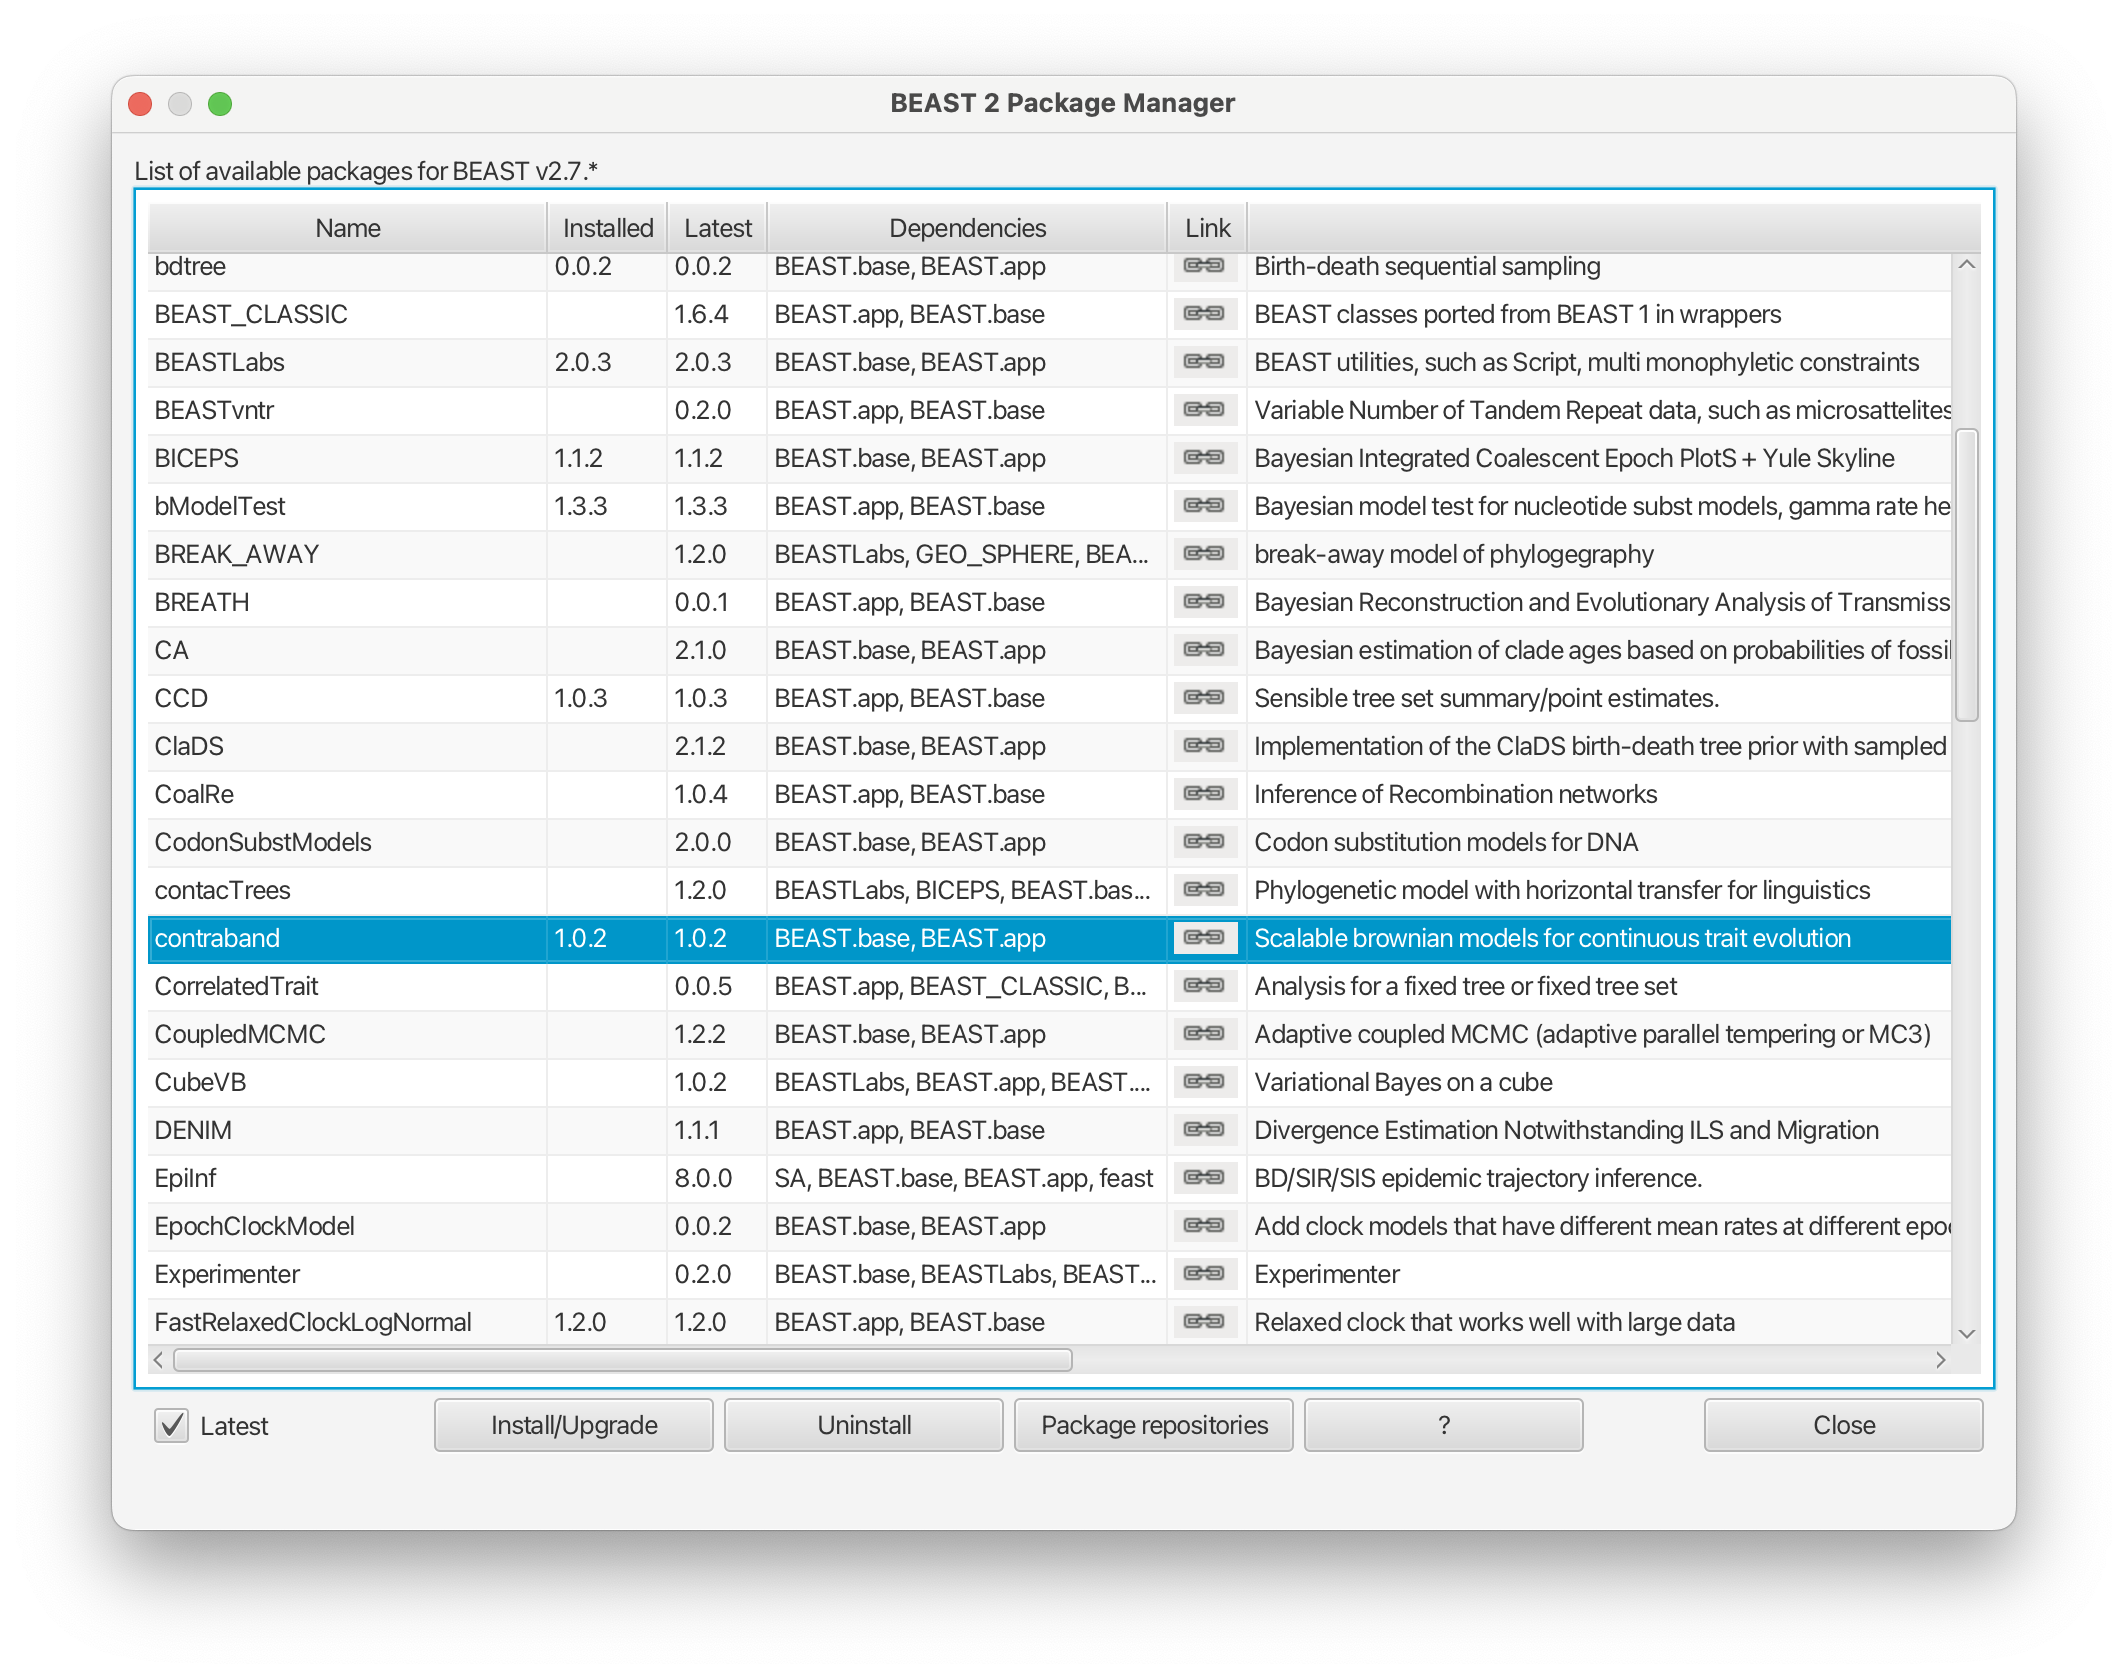
\includegraphics[width=0.5\textwidth]{figures/contrabandDownload.png}
    \caption{Downloading the \texttt{contraband} package.}
    \label{fig:example1}
\end{figure}

This tutorial will also make use of a few other packages;
these are \texttt{sampled-ancestors} and \texttt{morph-models}.
The first implements speciation and fossilization models (for evaluating the probability of phylogenies themselves), and the second implements models for the evolution of discrete morphological characters.
%These packages have a dedicated tutorial (here \textcolor{red}{[https://taming-the-beast.org/tutorials/Total-Evidence-Tutorial/]}) and will not be discussed further in the present exercise.
The SA and MM packages have two dedicated tutorials on the Taming the BEAST website (\href{https://taming-the-beast.org/tutorials/FBD-tutorial/}{here} and \href{https://taming-the-beast.org/tutorials/Total-Evidence-Tutorial/}{here}) and will not be discussed further in the present exercise.
The newly installed packages will become available in BEAUti2 once you close and restart the program.

\subsection{The data}

The data sets used in this tutorial include three types of data -- molecular, discrete morphology and continuous morphology -- scored for up to 27 carnivore species (11 of which are extinct and 16 of which are extant).

\subsubsection{Continuous characters}
Our TED analysis will leverage a published geometric-morphometric data set consisting of 29 three-dimensional (3D) cranium landmarks \citep{alvarez19}, each dimension of which will be treated as a separate continuous character (i.e., we will have a total of 87 continuous characters).
This data can be found in file \texttt{carnivora\_continuous\_27.nex} attached to this tutorial.

The same cranium landmarks have also been scored in 21 \textit{Vulpes vulpes} (one of the focal carnivore species) individuals.
This intraspecific data will be used in the analyses to bypass the estimation of character correlations ($\boldsymbol{\rho}$), and can be found in the attached file \texttt{vulpes\_continuous\_data.txt}.

\subsubsection{Discrete characters}
%In addition to continuous characters, our data set includes discrete morphological characters, scored in 12 of the carnivoran species.
%These discrete morphological characters describe these species' basicranial, dental, postcranial anatomical features (\texttt{carnivora\_discrete\_27.nex}) \citep{barrett21}.
%There are 183 characters in total and the number of character states ranges from 0 to 3. 
12 species of interest have discrete morphological characters that describe their basicranial, dental and postcranial anatomical features (\texttt{carnivora\_discrete\_27.nex}) \citep{barrett21}. There are 183 features in total and the number of character states ranges from 0 to 3. 

\subsubsection{Molecular sequences}
%Finally, we will use molecular sequences of 12 mitochondrial genes obtained for 14 carnivoran species on NCBI.
%These sequences have been aligned and concatenated (\texttt{carnivora\_dna\_27.fasta}).
The molecular sequences of 12 mitochondrial genes for 14 species of interest were collected from the NCBI database, concatenated and aligned using MAFFT (\texttt{carnivora\_dna\_27.fasta}).

\section{Practical part \uppercase\expandafter{\romannumeral 1}: Bayesian phylogenetic inference using multiple continuous morphological characters}

The following section shall carry out Bayesian inference of divergence times using continuous morphology only; the main player here is the Brownian model implemented in the \texttt{contraband} package.

Like in other tutorials, we will use BEAUti2 as a tool for specifying BEAST2 .XML files for running our analyses.

\subsection{Setting up the analysis in BEAUti}
\subsubsection{Loading the Carnivoran Continuous data}\label{load-continuous-data}

We start by opening BEAUti2 and loading the continuous morphology data available for our carnivoran species.
This data can be found in \texttt{data/carnivora\_continuous\_27.nex}.
You can then either drag and drop that file into BEAUti2's ``Partitions'' panel, or use the system's drop-down menu and do File > Load Continuous Data.
Once the data is loaded successfully into BEAUTi 2, you should be able to see it in the updated ``Partitions'' panel.

\begin{figure}[!htbp]
    \centering
    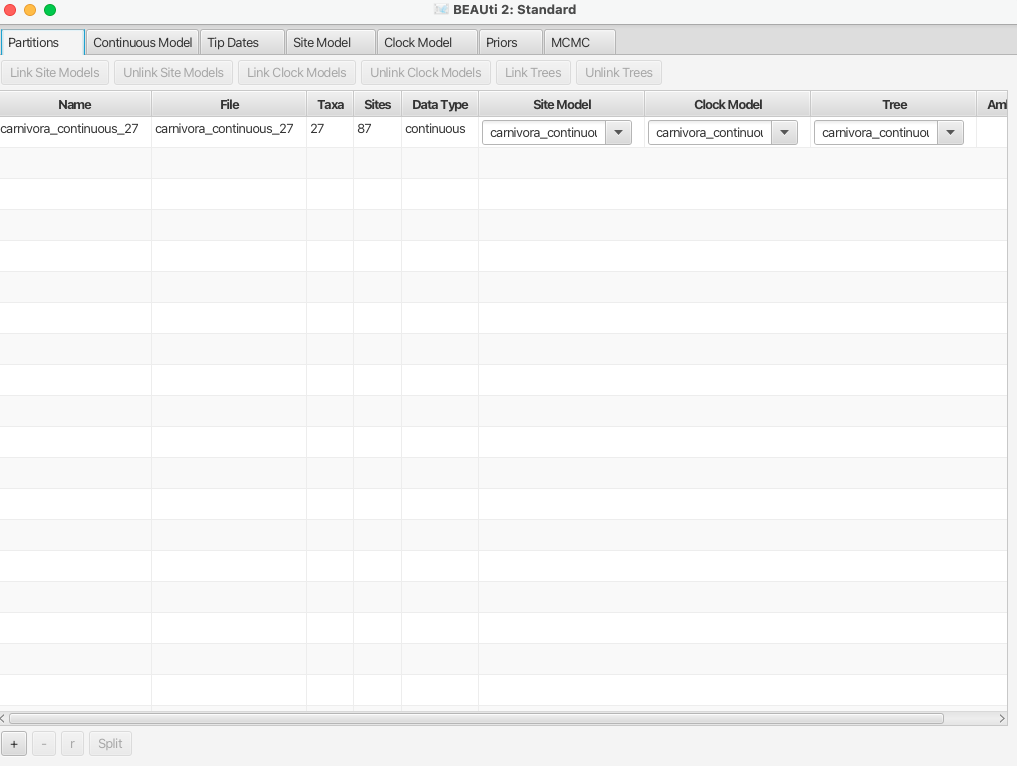
\includegraphics[width=0.700000\textwidth]{figures/BMPartition.png}
    \caption{Loading the continuous data.}
    \label{fig:example0}
\end{figure}

\subsubsection{Get the fossil ages (tip dates)}\label{parse-fosill-age}

Some of the species (i.e., terminal nodes, or ``tips'') in our tree are extinct and we will assume their ages are known (from dating their fossils) without error.
How to relax this assumption appropriately is an active area of research that is outside the scope of this tutorial.

In order to set the age of these tips, open the ``Tip Dates'' panel and check ``Use tip dates''.
Inputting tip dates can be done in multiple ways, but in our case, fossil ages are provided as part of each species name, after the second underscore ``\texttt{\_}''.
Conveniently, BEAUti2 can deal with those if we click the ``Auto-configure'' button.
Select ``use everything'', then select ``after last'' from the drop-down box to the right, and input ``\texttt{\_}'' (without quotes) in the text box immediately to the right (\autoref{fig:example2}).
Clicking ``Ok'' should now populate the table with the fossil ages extracted from the species names.

\begin{figure}[!htbp]
    \centering
    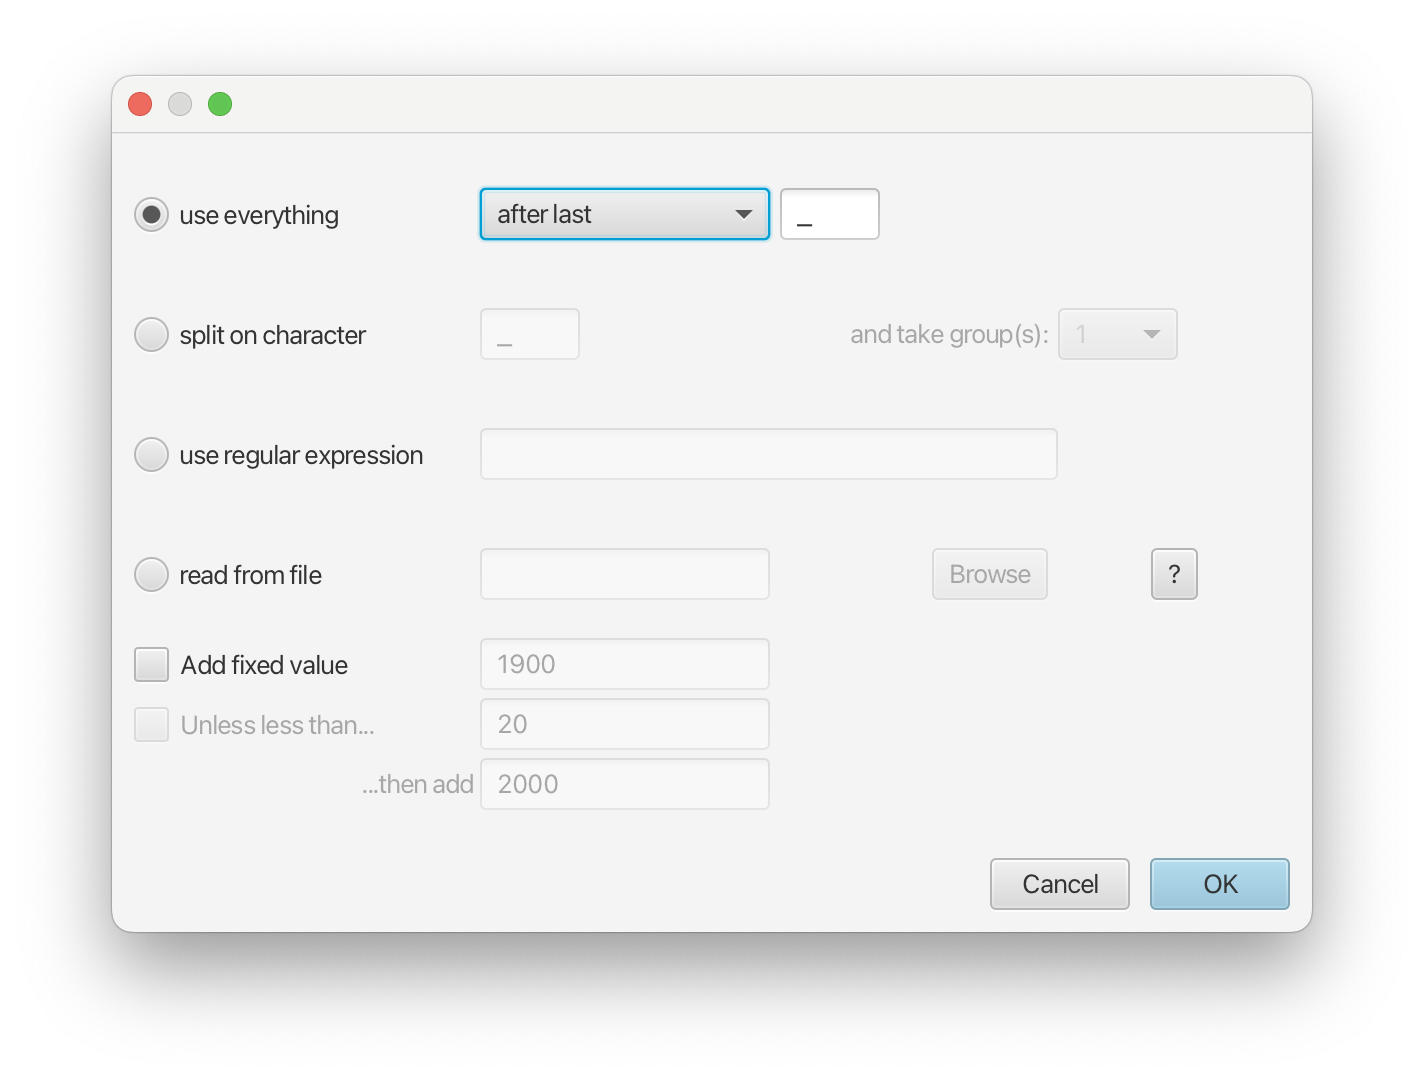
\includegraphics[width=0.5\textwidth]{figures/BMParseDates.png}
   \caption{Guessing sampling times.}
    \label{fig:example2}
\end{figure}

In the populated table (\autoref{fig:example3}), columns \textbf{Date} and \textbf{Age/Height} should now have values between 0.0 and 35.55 million years.
Note how living species have ages of 0.0 and extinct species have ages > 0.0.

\begin{figure}[!htbp]
    \centering
    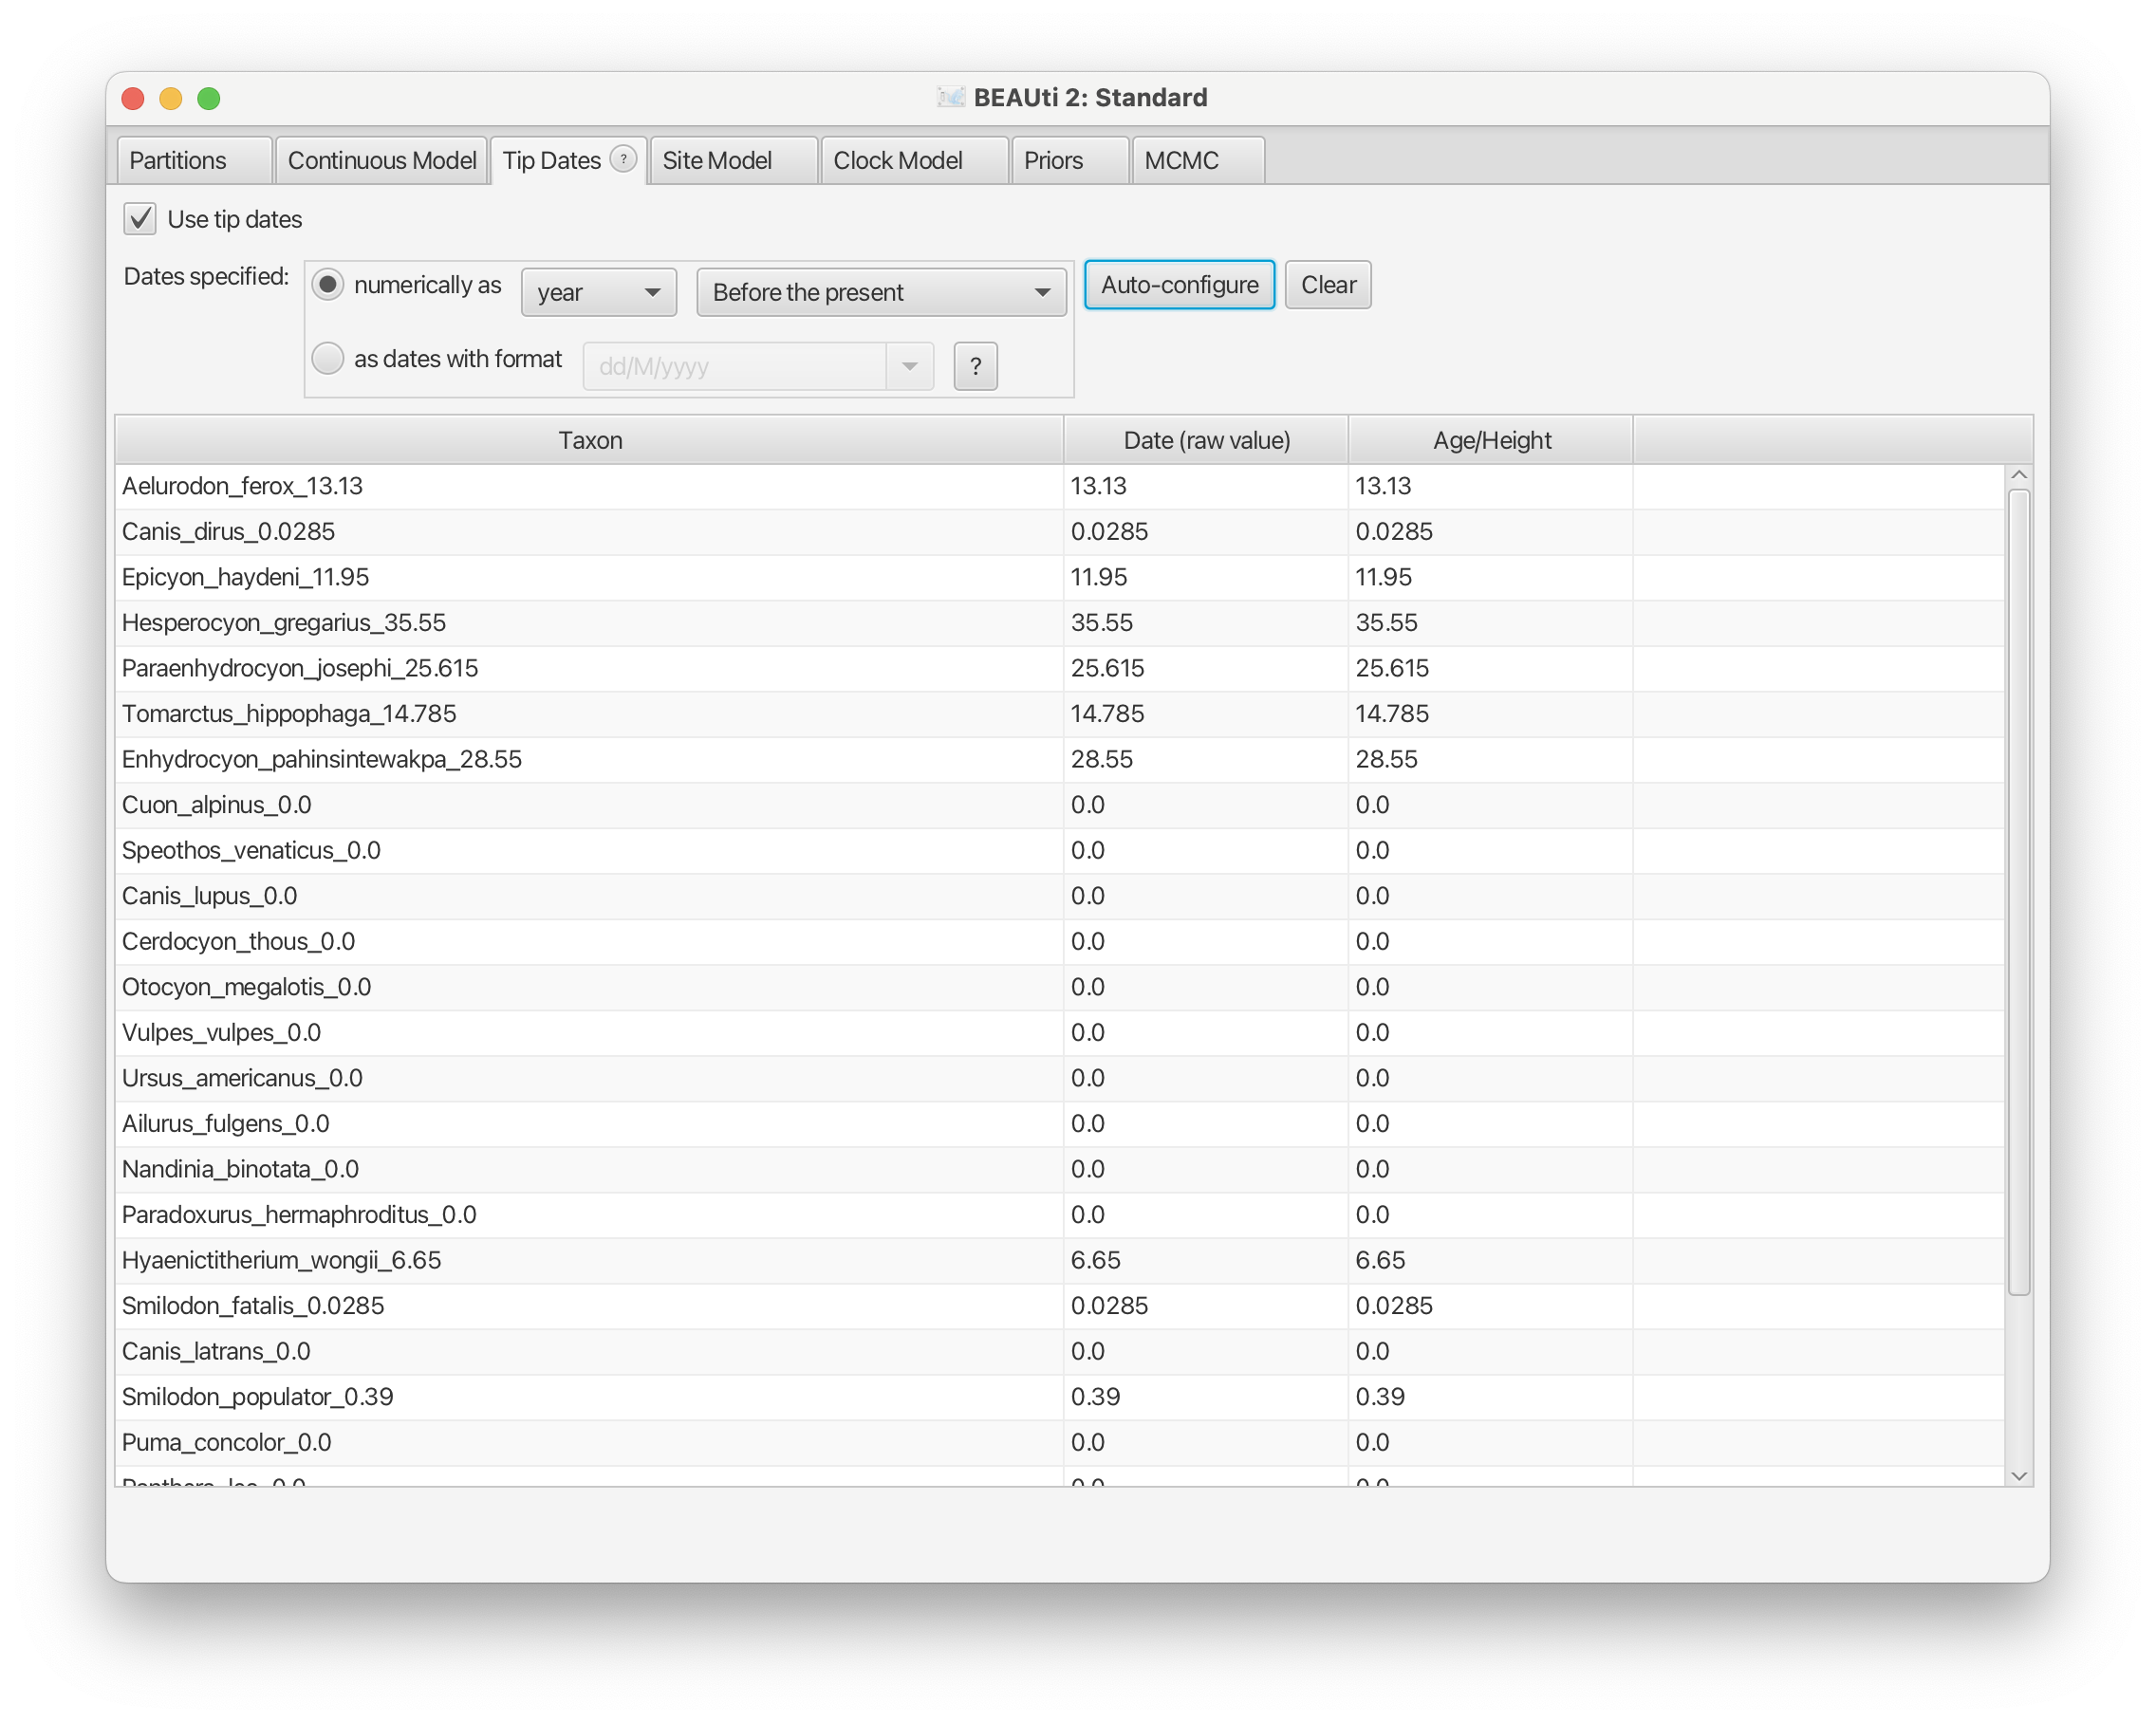
\includegraphics[width=0.700000\textwidth]{figures/BMTipDates.png}
    \caption{Fossil ages.}
    \label{fig:example3}
\end{figure}

\subsubsection{Setting up the Brownian motion model}

As elaborated in the background section above, there are a few key Brownian motion model parameters that concern us.
Namely:\begin{enumerate}\item the character values at the root of the tree, $\boldsymbol{y_0}$, \item the character correlations, $\boldsymbol{\rho}$, and \item the character-specific evolutionary rates, $\boldsymbol{r}$.\end{enumerate}

We want to estimate all these parameters (so check all the ``estimate'' boxes), but for simplicity, we will assume that all characters are evolving at the same relative rate.
Therefore, we want to check the ``One Rate Only'' box.
Parameter values at the start of the MCMC chain can be specified in the text boxes next to their corresponding parameters names; these should not matter for analysis convergence, and we will just use arbitrary, round values (Fig. \ref{fig:example4}).

\begin{figure}[!htbp]
    \centering
    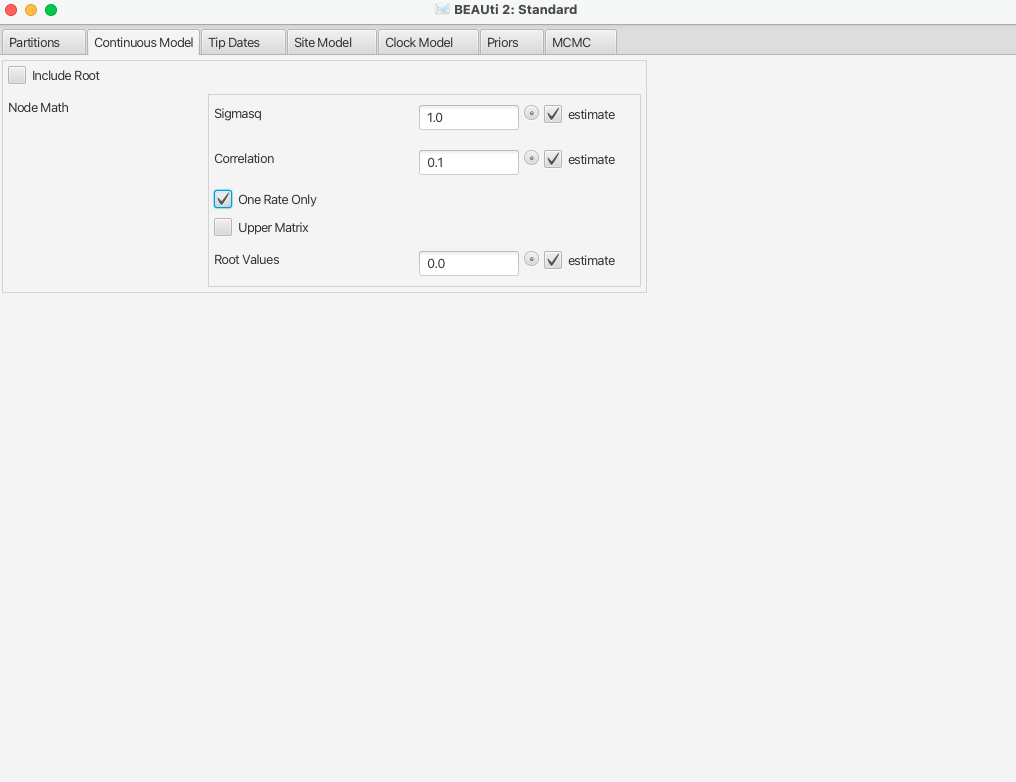
\includegraphics[width=0.700000\textwidth]{figures/BMModel.png}
    \caption{BM model parameter specifications.}
    \label{fig:example4}
\end{figure}

\subsubsection{Setting up the morphological clock model}\label{bm-clock-model}

In addition to character-specific morphological rates, the morphological clock model we will use has two components: a global rate, $c_m$, and branch-specific relative rates, $\boldsymbol{b_m}$.
The total rate for a branch $i$ and a character $k$ is given by $c_m \times \boldsymbol{b_m}^i \times \boldsymbol{r}^k$ (with superscript indexing vectors).
Note that once $c_m$ is assigned an absolute value, the branch-specific rates (as well as character-specific rates) must be relative.
(For the same product of rates and a given $c_m$, there is an infinite number of combinations of $\boldsymbol{b_m}^i$ and $\boldsymbol{r}^k$.)

In order to set up the morphological clock model, click the ``Clock Model'' tab, and choose the relaxed uncorrelated clock.
The ``Mean clock rate'' stands for the global morphological rate, $c_m$ -- we want to estimate it (leave the ``estimate'' checkbox ticked) and initialize it to 1.0.
Note that the actual mean of the log-normal distribution characterizing the relaxed clock is a separate parameter set by BEAUti2 automatically to 1.0, which makes branch-specific rates relative.
All other clock parameters are also automatically set by BEAUti2.

\begin{figure}[!htbp]
    \centering
    \includegraphics[width=0.700000\textwidth]{figures/BMucln.png}
    \caption{Choosing the relaxed uncorrelated clock model and initializing $c_m$.}
    \label{fig:example5}
\end{figure}

\subsubsection{Specifying prior models}

Considering our prior beliefs about parameter values is a key ingredient of Bayesian statistics.
We will do so by assigning prior distributions to each parameter in the ``Priors'' tabs.

The key prior specification we want to do is assigning the fossilized birth-death (FBD) model \citep{gavryushkina2014} as the prior distribution for our Carnivora species tree.
All the other parameters will be assigned default prior distributions by BEAUti2; we will have to modify some of these by hand directly on the .XML produced by BEAUti2 (see disclaimer at the top of this document).

\begin{figure}[!htbp]
    \centering
    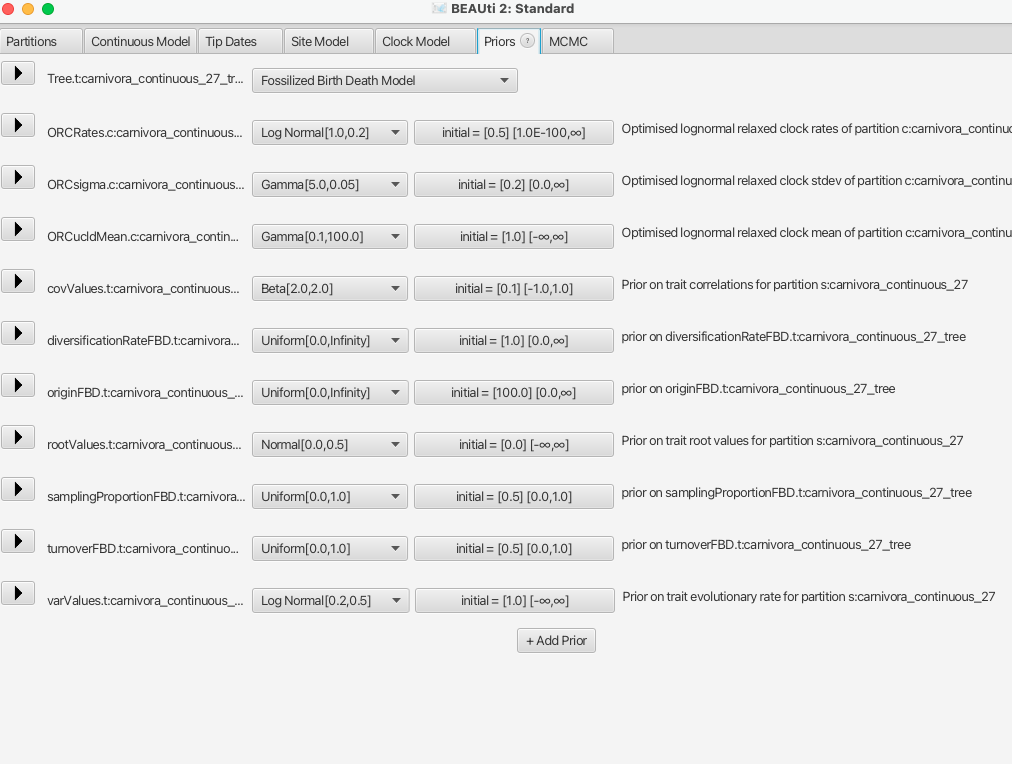
\includegraphics[width=0.700000\textwidth]{figures/BMPriors.png}
    \caption{Specifying prior distributions for the different model parameters.}
    \label{fig:example6}
\end{figure}

\subsubsection{MCMC chain configuration}\label{specify-the-mcmc-chain-length-mcmc}

Now we will configure our MCMC chain.
For this dataset, 2 million iterations should be sufficient to obtain large enough effective sample sizes (ESSs), and we will log every 2000 iterations (i.e., we will have 1001 samples in our log files).

Finally, we shall save our analysis configuration to an \texttt{.xml} file to to be run by BEAST2.
Click \emph{File \textgreater{}\textgreater{} Save as}, and choose a name for it.

\begin{figure}[!htbp]
    \centering
    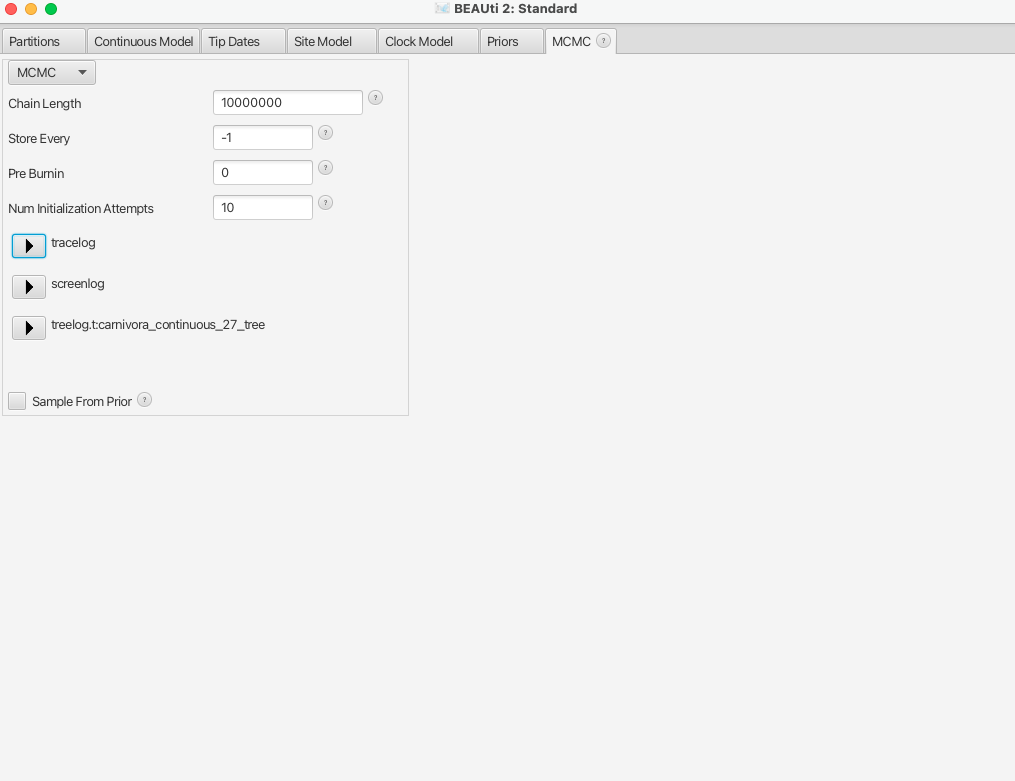
\includegraphics[width=0.700000\textwidth]{figures/BMMCMC.png}
    \caption{Configuring the length of the Markov chain as well as logging frequency.}
    \label{fig:example7}
\end{figure}

\subsubsection{Run the Analysis using BEAST2}\label{run-the-analysis-using-beast2}

It should be possible to now run our analysis by giving BEAST2 the \texttt{.xml} as done in other tutorial analyses.

\subsubsection{Processing the results}

Convergence of the Markov chain initiated by running the \texttt{.xml} generated above will take a long while, so we will processes the results of a precooked run (in the \texttt{precooked-runs/} directory).
In fact, this precooked run was also not run for very long, as you will see.
Open the Tracer application and load file ``BM.log".

The first thing we will note is that the ESS values are all below 200 and shown in red (\autoref{fig:bm_res1}) -- obviously our Markov chain needs to run for much longer for us to safely conclude anything about the biological system we are studying.

\begin{figure}[!htbp]
    \centering
    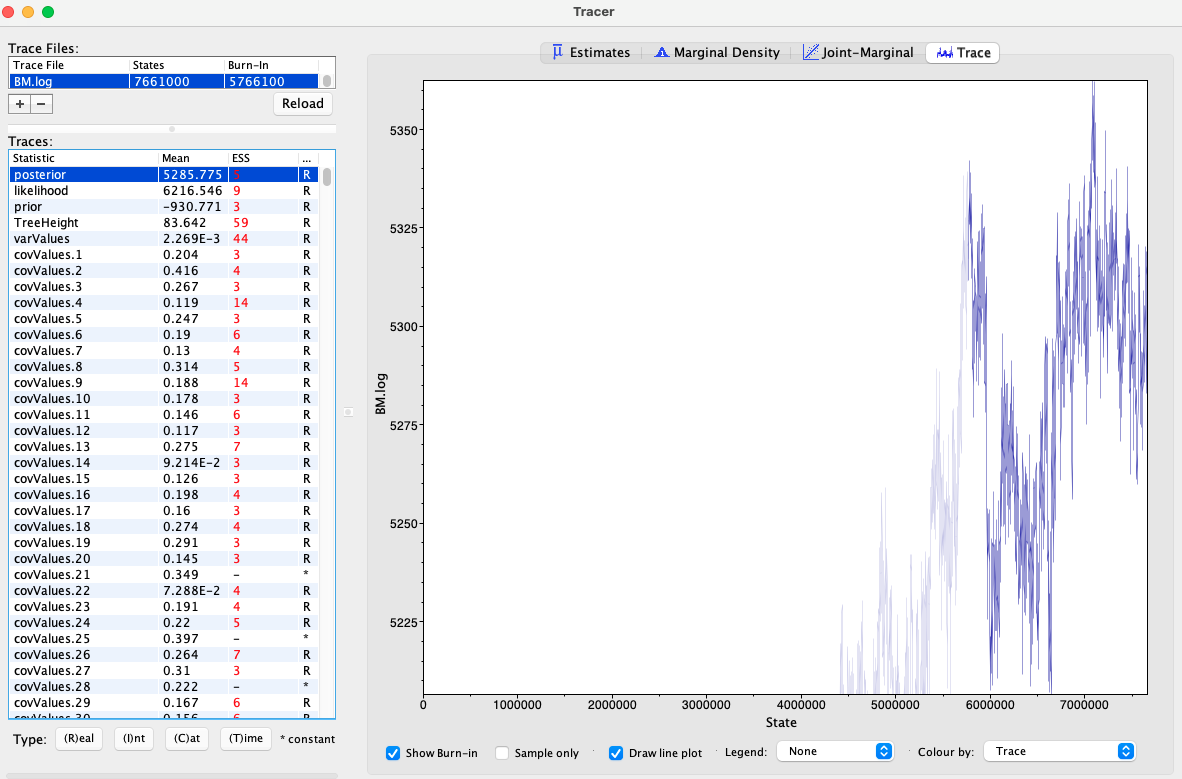
\includegraphics[width=0.700000\textwidth]{figures/results/BM_posterior.png}
    \caption{Visualizing effective sample sizes (ESSs) of different parameters on Tracer.}
    \label{fig:bm_res1}
\end{figure}

We can, however, navigate through the parameters shown by Tracer.
If the \texttt{.log} file were to be updated by an active BEAST2 process, one could click ``Reload'' the file and see how parameter values change (or not) as the Markov chain approaches convergence.

\clearpage

The parameters we can track on Tracer are the global morphological clock rate, $c_m$ (\autoref{fig:bm_res5}),

\begin{figure}[!htbp]
    \centering
    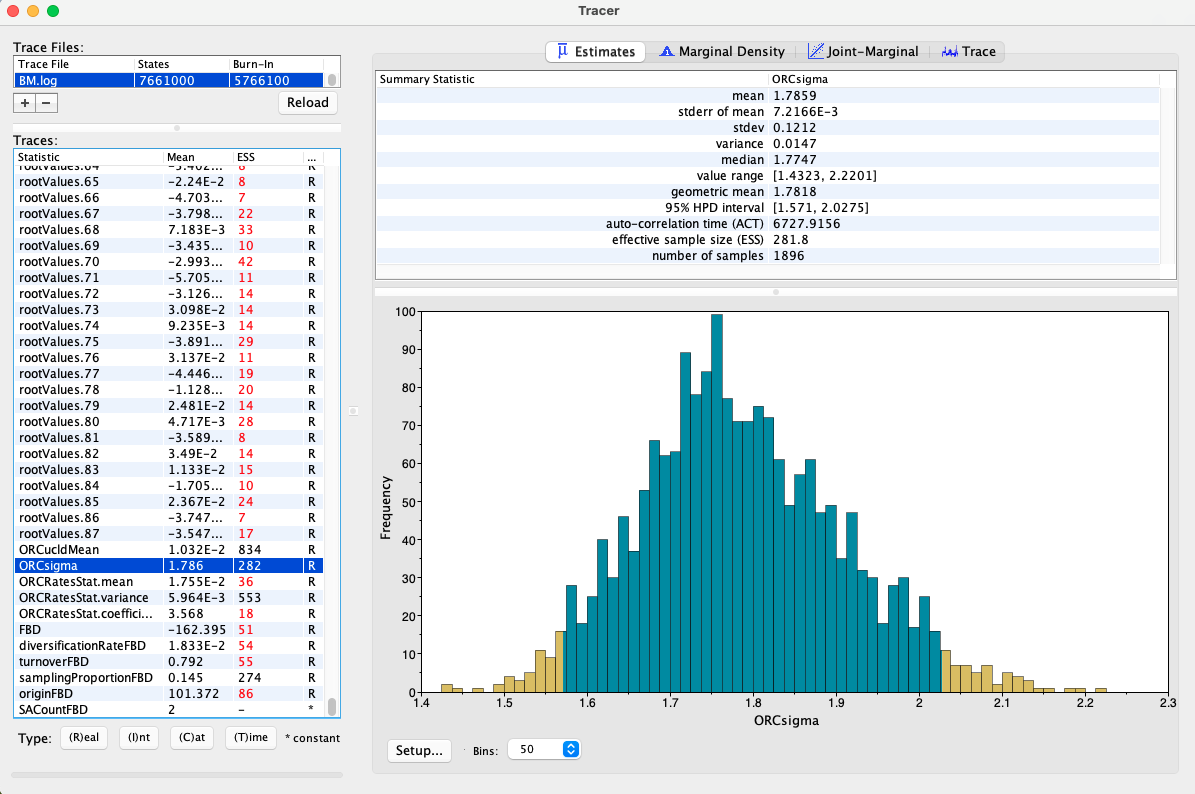
\includegraphics[width=0.700000\textwidth]{figures/results/BM_clock_sigma.png}
    \caption{Posterior distribution of the global morphological clock rate, $c_m$.}
    \label{fig:bm_res5}
\end{figure}

\noindent the character-specific relative evolutionary rate, $\boldsymbol{r}$ (in this case shared by all characters; \autoref{fig:bm_res2}),

\begin{figure}[!htbp]
    \centering
    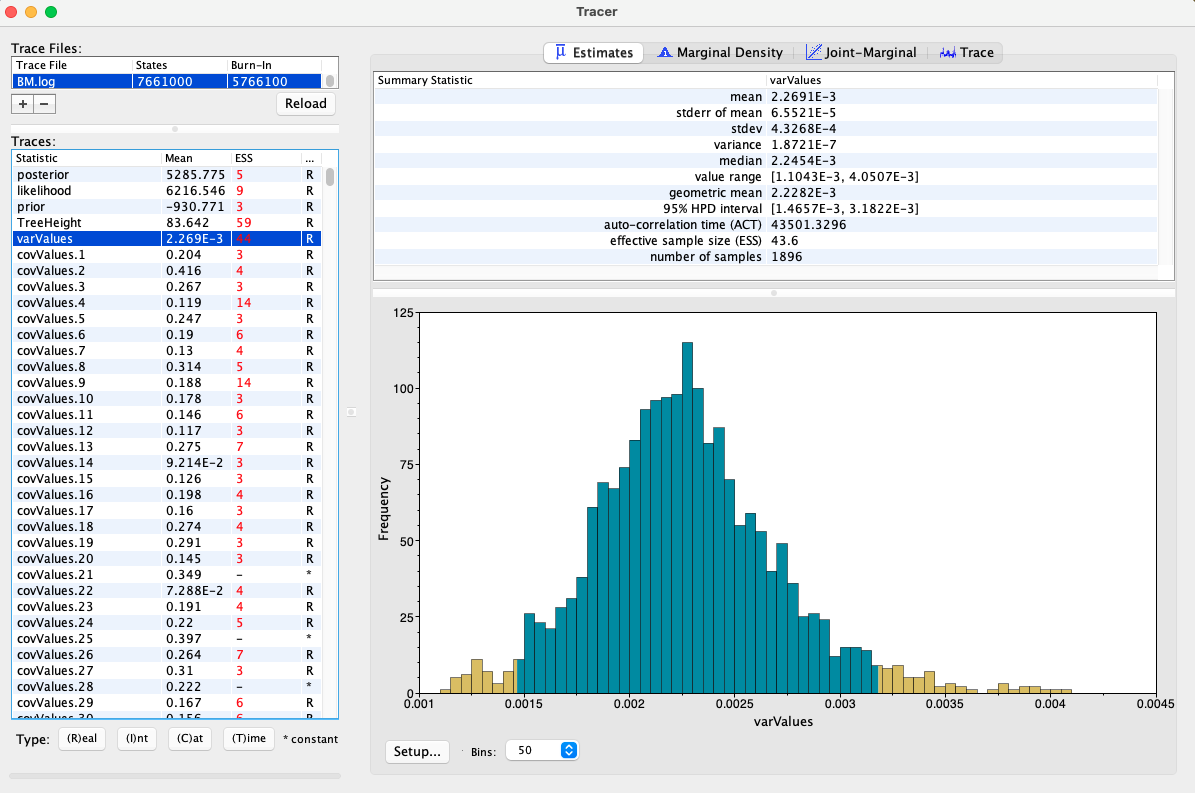
\includegraphics[width=0.700000\textwidth]{figures/results/BM_evo_rate.png}
    \caption{Posterior distribution of character-specific relative evolutionary rate (in this case shared by all 87 characters).}
    \label{fig:bm_res2}
\end{figure}

\clearpage

\noindent the between-character correlations, $\boldsymbol{\rho}$ (\autoref{fig:bm_res3}),

\begin{figure}[!htbp]
    \centering
    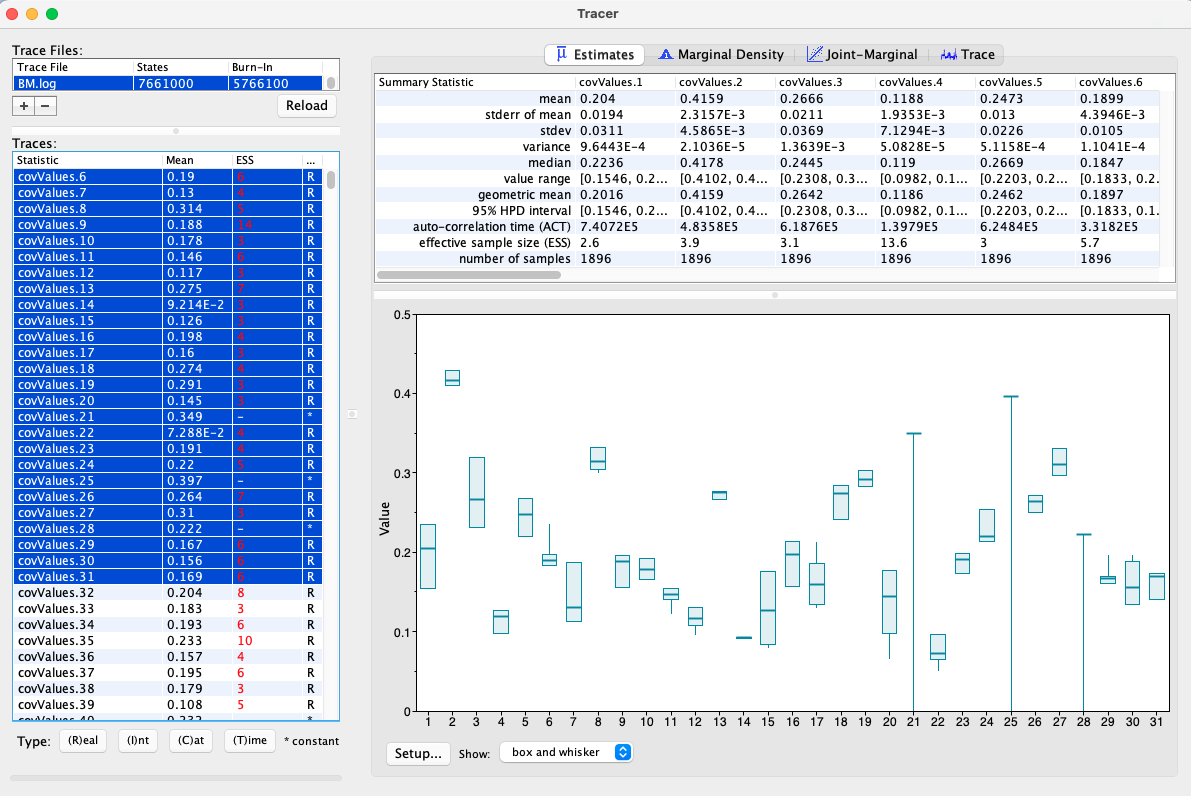
\includegraphics[width=0.700000\textwidth]{figures/results/BM_covValues.png}
    \caption{Posterior distribution of the between-character correlations.}
    \label{fig:bm_res3}
\end{figure}

\noindent and the character states at the root of the tree, $\boldsymbol{y_0}$,

\begin{figure}[!htbp]
    \centering
    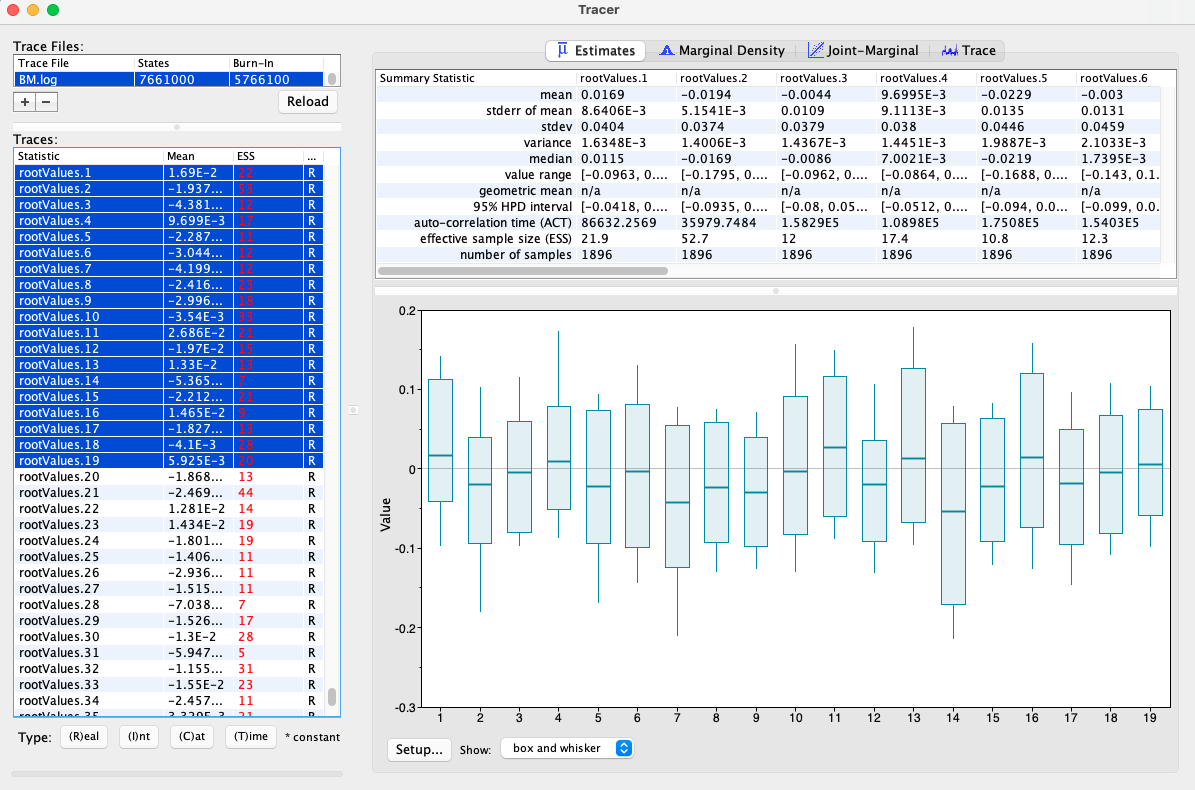
\includegraphics[width=0.700000\textwidth]{figures/results/BM_rootValues.png}
    \caption{87 trait values at the root of the tree.}
    \label{fig:bm_res4}
\end{figure}

\clearpage

The last thing we will do is something you will have likely done before in other tutorials: obtaining and visualizing a summary of the posterior distribution of trees.
Open TreeAnnotator, and leave ``Burn in percentage'', ``Target tree type'' and ``Node heights'' at their default values.
Then for ``Input Tree File'', choose \texttt{precooked\_runs/carnivora\_continuous\_27\_tree\_bm.trees}, and for ``Output File'', type \texttt{carnivora\_continuous\_27\_bm\_mcc.tree}.
Then click ``Run'' to summarize the tree posterior distribution into a maximum-clade-credibility (MCC) tree. 

After this, the summary tree generated by TreeAnnotator can be visualized in FigTree (\autoref{fig:bm_res6})

\begin{figure}[!htbp]
    \centering
    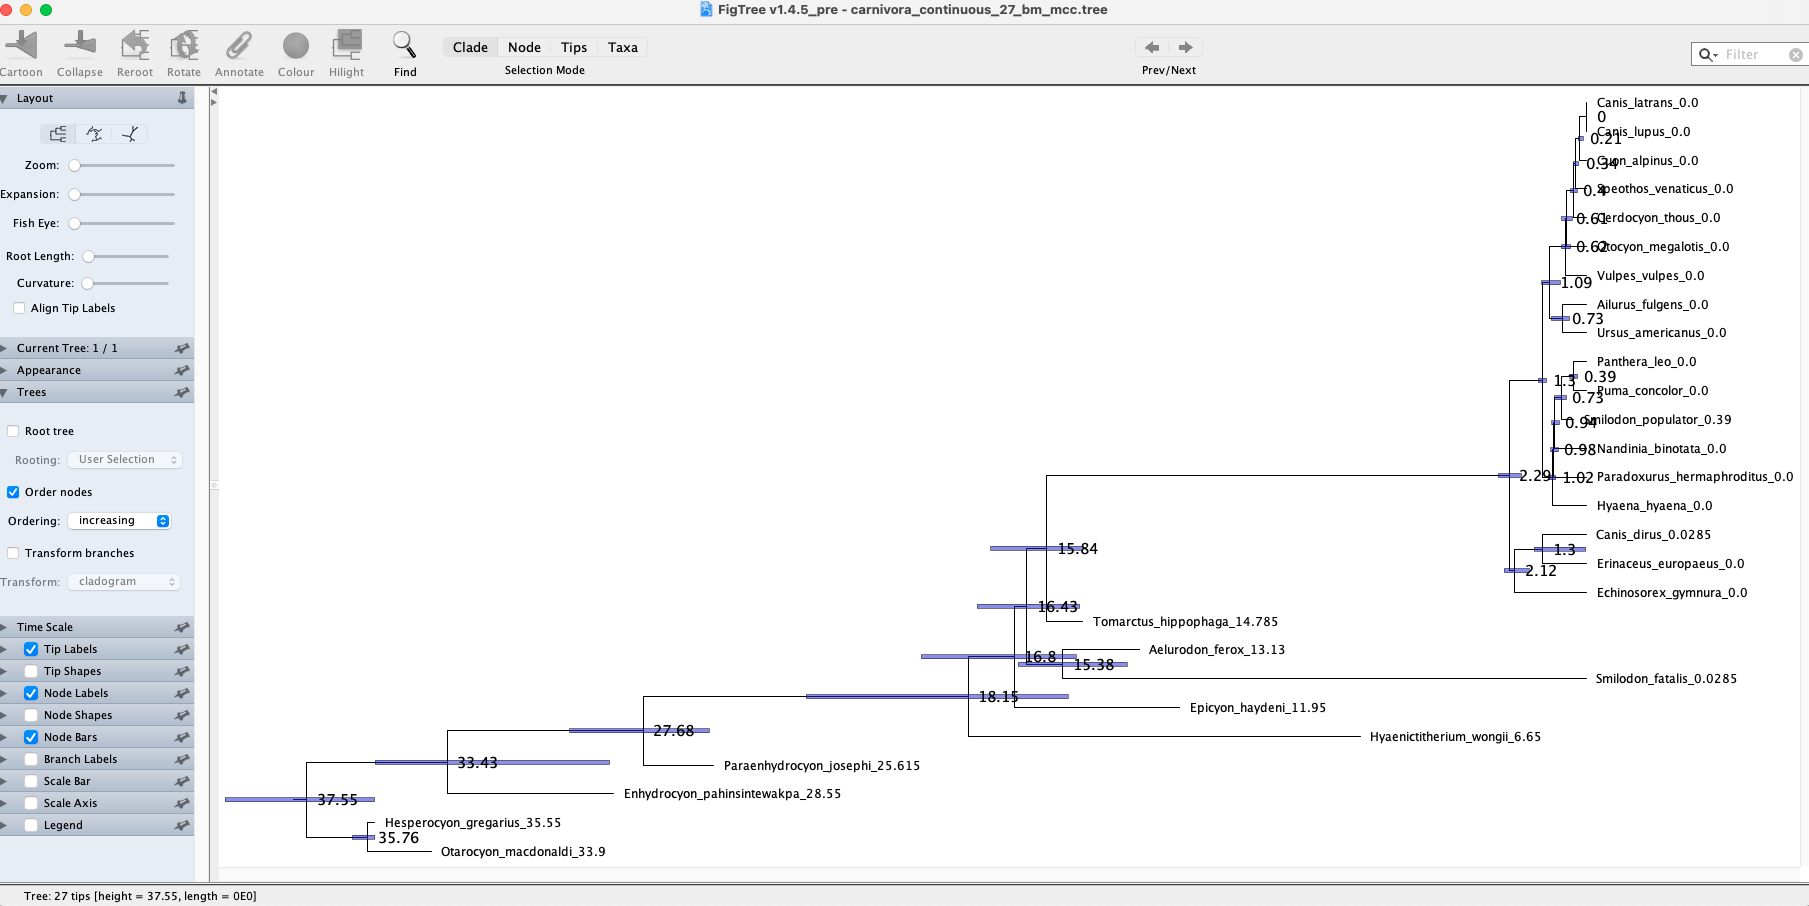
\includegraphics[width=0.700000\textwidth]{figures/results/BM_MCC_tree.png}
    \caption{Maximum-clade-credibility tree summarized from posterior distribution of trees.}
    \label{fig:bm_res6}
\end{figure}

This MCC tree (\autoref{fig:bm_res6}) has been estimated using multiple correlated continuous characters and nothing else!

\section{Practical part \uppercase\expandafter{\romannumeral 2}: Total-evidence dating using multiple continuous morphological characters (and more!)}

In the following section, we will set up an integrative model with components for each type of data (described above) -- this will be a full-blown total-evidence dating analysis with all the data we have.

Like in other tutorials, we will use BEAUti2 as a tool for specifying BEAST2 .XML files for running our analyses.

\subsection{Setting up the analysis in BEAUti}

\subsubsection{Loading the Carnivoran data sets}
We first load the continuous data and parse the fossil ages as in sections~\ref{load-continuous-data} and~\ref{parse-fosill-age}. Then, in the "Partitions" panel, we also load the Carnivoran molecular sequences via \emph{File \textgreater{}\textgreater{} Import Alignment}. Finally, we add the discrete characters by \emph{File \textgreater{}\textgreater{} Add Morphological Data}. As is shown in \autoref{fig:example8}, the two rows with "nucleotide" as Data Type indicate that the molecular sequences are partitioned based on the codon positions, i.e., first and second codon positions for the first partition and the third codon positions for the second partition. Likewise, the last  three rows with "standard" as Data Type indicate that the discrete data are partitioned based on the number of states the characters have. In this data set, the discrete characters are described by the states the number of which ranges from 2 to 4.  

\begin{figure}
    \centering
    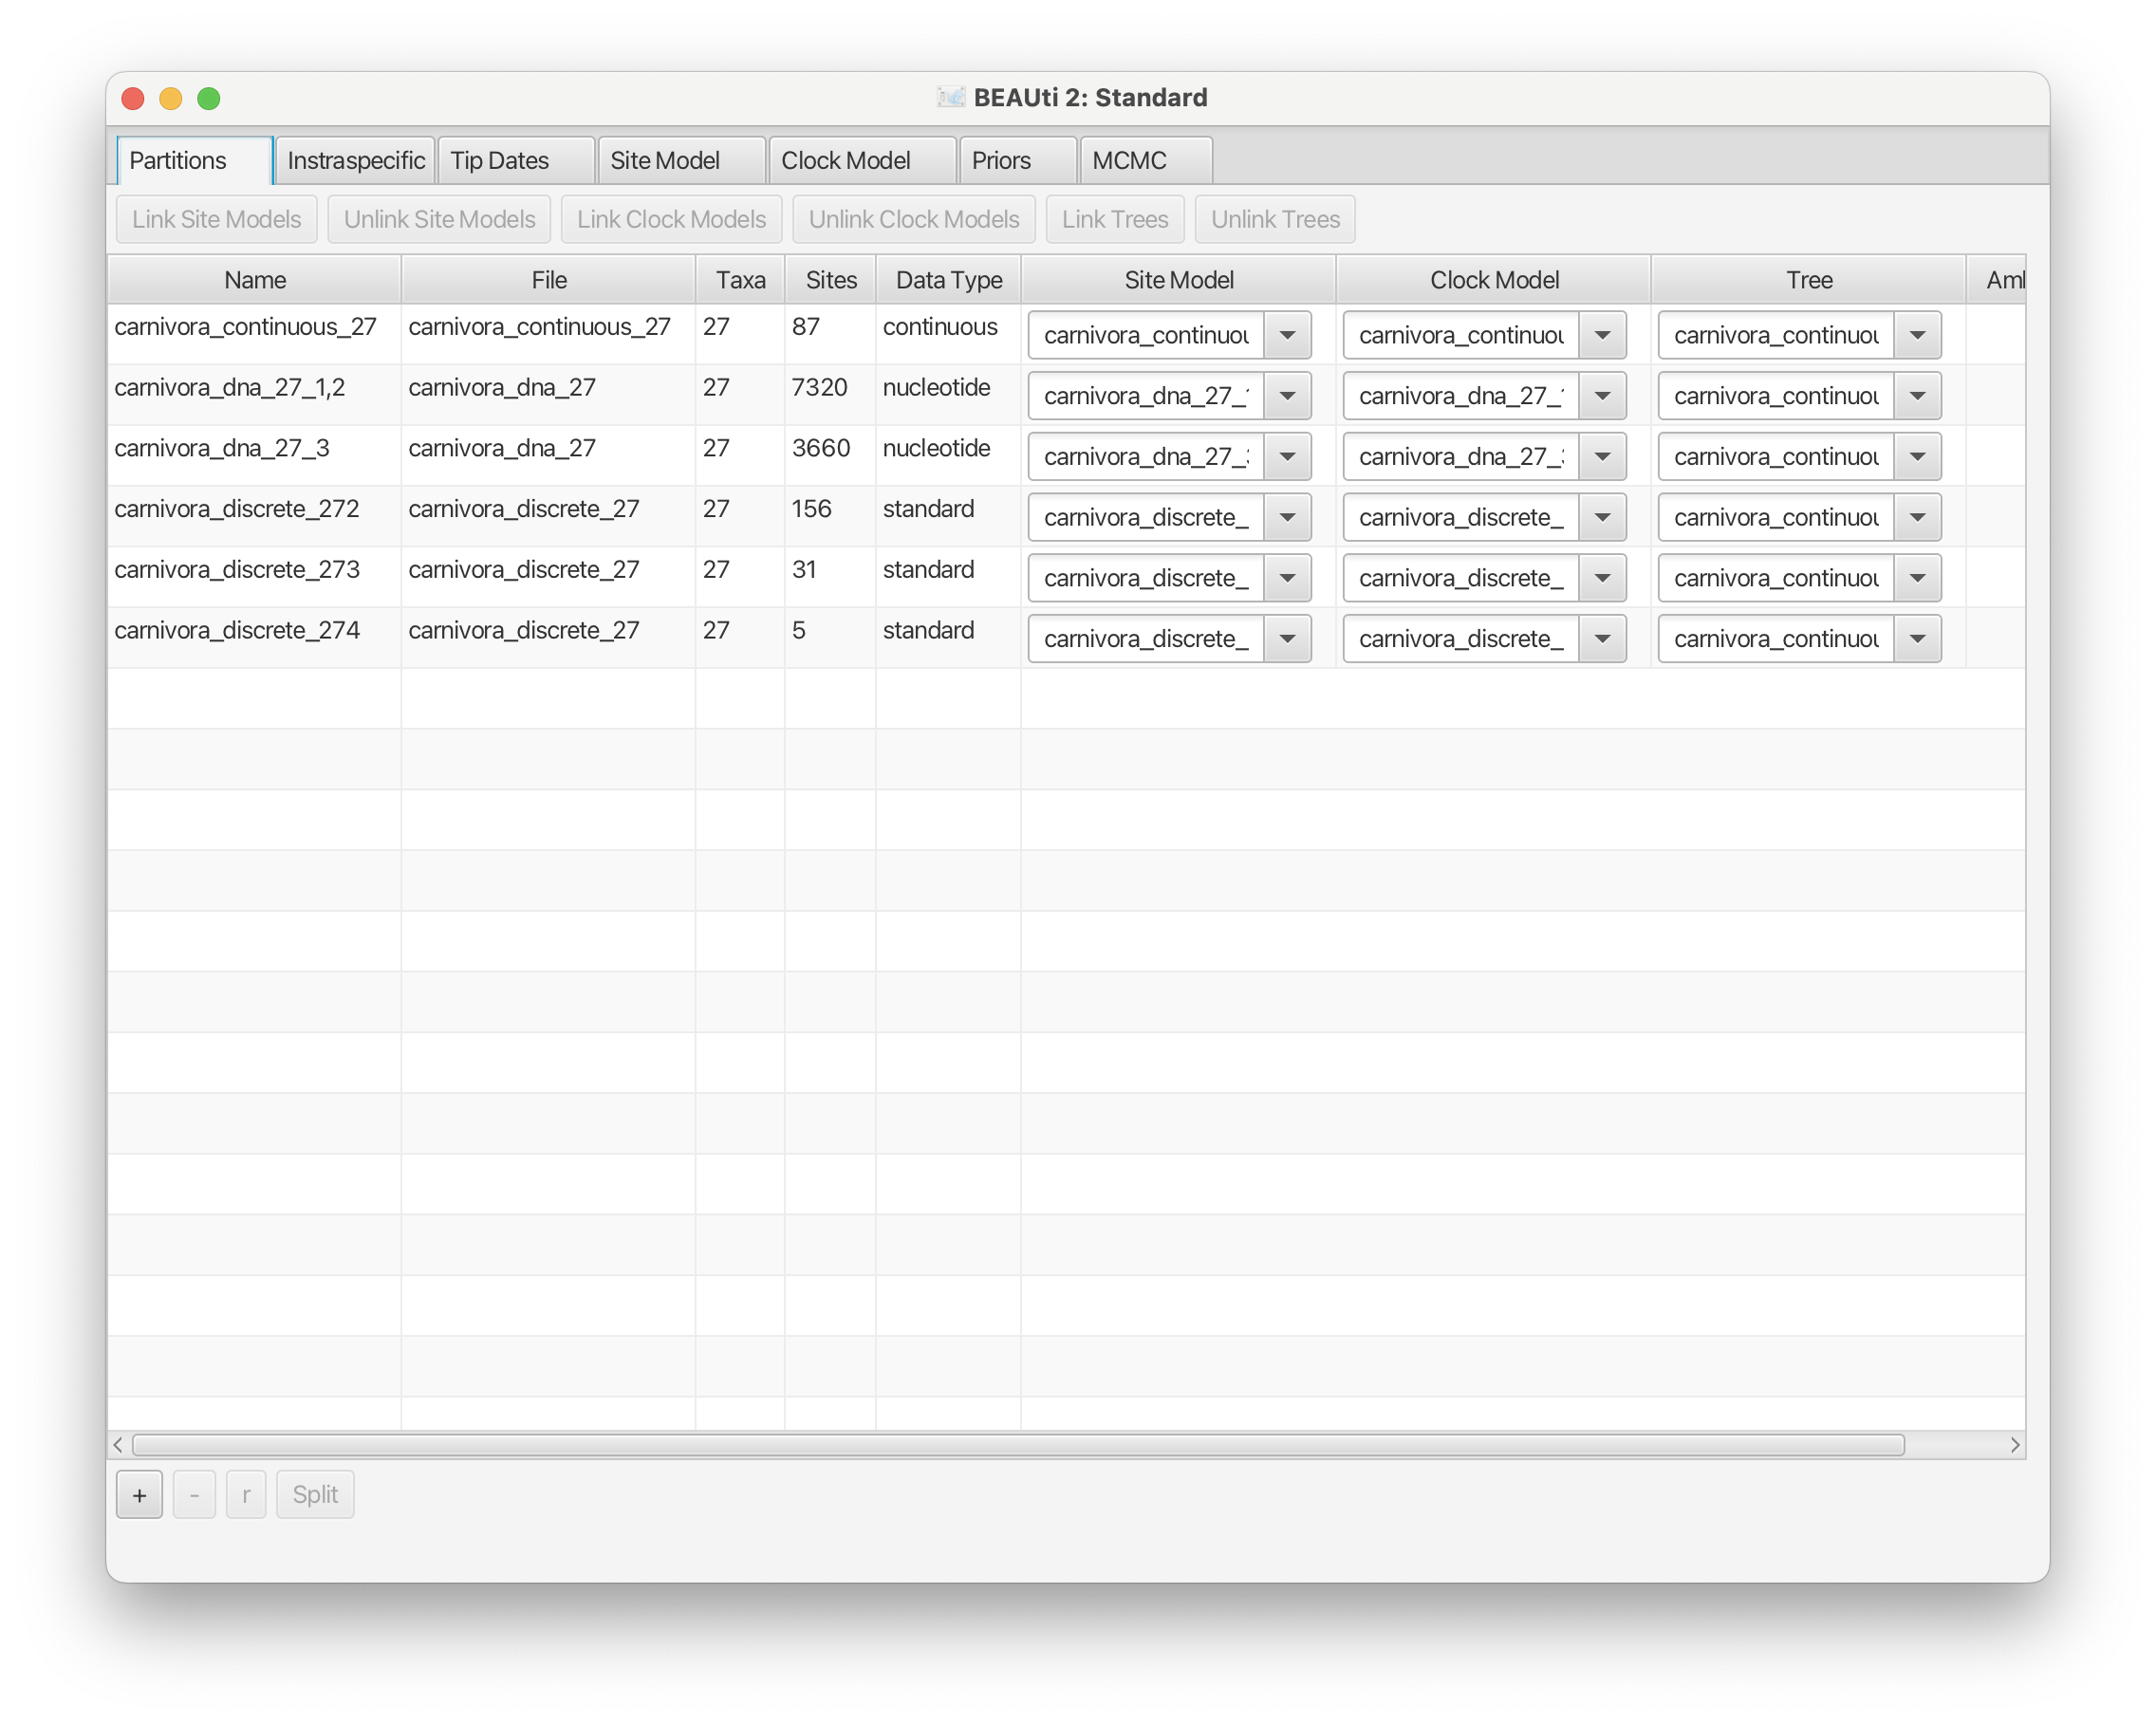
\includegraphics[width=0.700000\textwidth]{figures/DataPartitions.png}
    \caption{Loading continuous characters, molecular sequences and discrete characters.}
    \label{fig:example8}
\end{figure}


%%\subsubsection{Set the Shrinkage Model}
%%In the "Shrinkage Model" panel, we will need to fill in three components of the model. First, the shrinkage parameter is given by a constant value in the box to the right of "Delta". Second, the continuous characters from 21 \textit{Vulpes vulpes} individuals are given in the block of "Population Traits". To be more specific, the trait data should be written in one-line data separated by spaces. In addition, the number of trait is given by "Minordimension" and should be consistent with the dimension of the continuous data in ''Partitions" panel. Third, the added individual trait values are not only used for estimating correlations, but also normalizing the continuous data of the 19 carnivoran species. Therefore, we put a $\checkmark$ in the box in front of "Include Pop Var". 
\subsubsection{Setting the Shrinkage Model}
In the "Shrinkage Model" panel, we will need to fill in three components of the model. First, the shrinkage parameter is given by a constant value in the box to the right of "Delta". Second, the continuous characters from 21 \textit{Vulpes vulpes} individuals are given in the block of "Population Traits". To be more specific, the trait data should be written in one-line data separated by spaces. In addition, the number of traits is given by "Minordimension" and should be consistent with the dimension of the continuous data in the ''Partitions" panel. Third, the added individual trait values are not only used for estimating correlations, but also normalizing the continuous data of the 19 carnivoran species. Therefore, we put a $\checkmark$ in the box in front of "Include Pop Var" (\autoref{fig:example9}). 

\begin{figure}[!htbp]
    \centering
    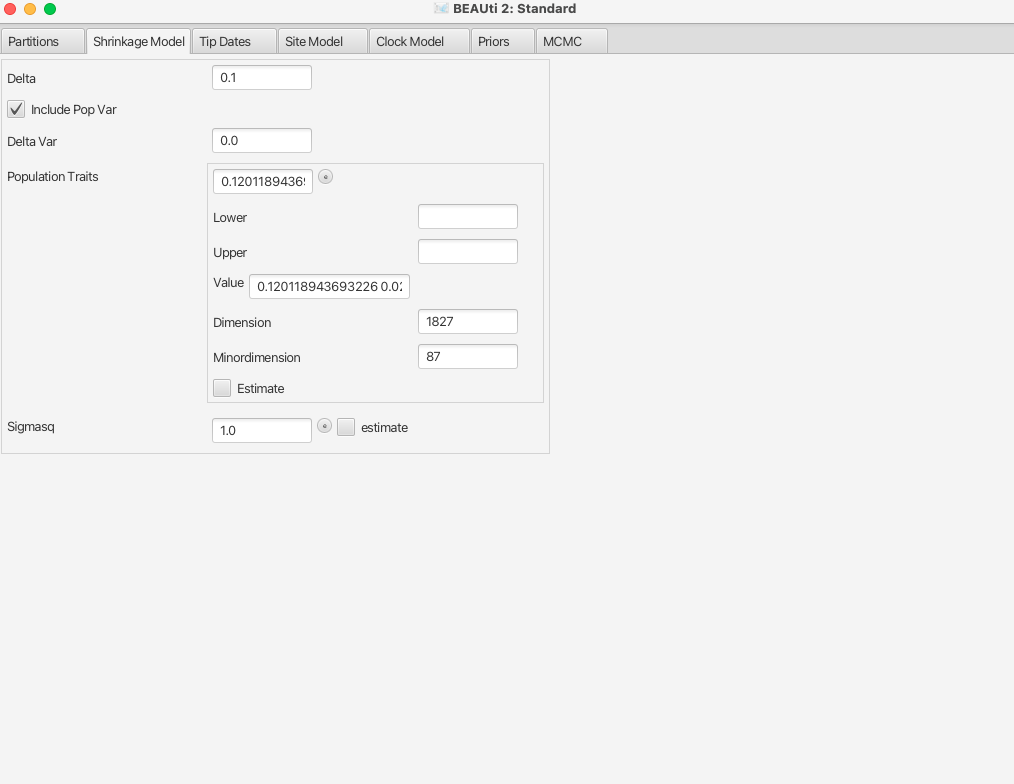
\includegraphics[width=0.700000\textwidth]{figures/ShrinkageModel.png}
    \caption{Setting the shrinkage model.}
    \label{fig:example9}
\end{figure}


\subsubsection{Setting the Substitution Model}
In the "Site Model" panel, we assume an HKY+Gamma model for nucleotide substitutions by specifying 4 categories under "Gamma Category Count" \autoref{fig:example10}. In addition, we assume Mk models  \citep{lewis2001} for the discrete characters, as is shown in \autoref{fig:example11}.

\begin{figure}[!htbp]
    \centering
    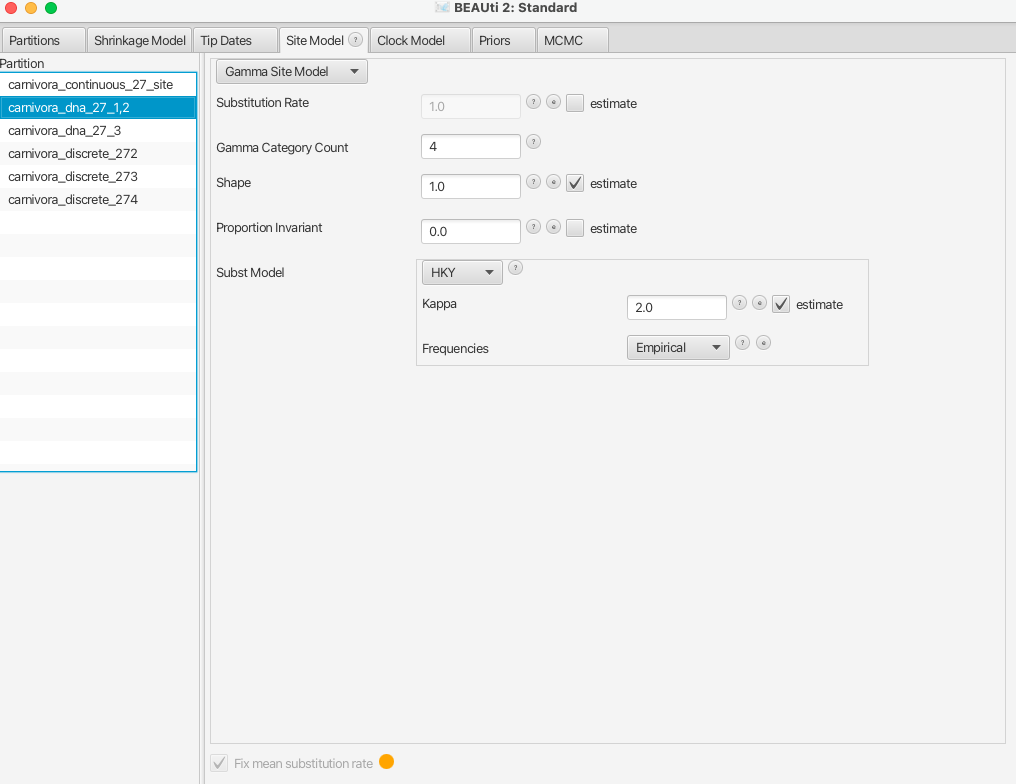
\includegraphics[width=0.700000\textwidth]{figures/SiteModelDNA.png}
    \caption{Setting site models for molecular sequences and discrete characters.}
    \label{fig:example10}
\end{figure}

\begin{figure}[!htbp]
    \centering
    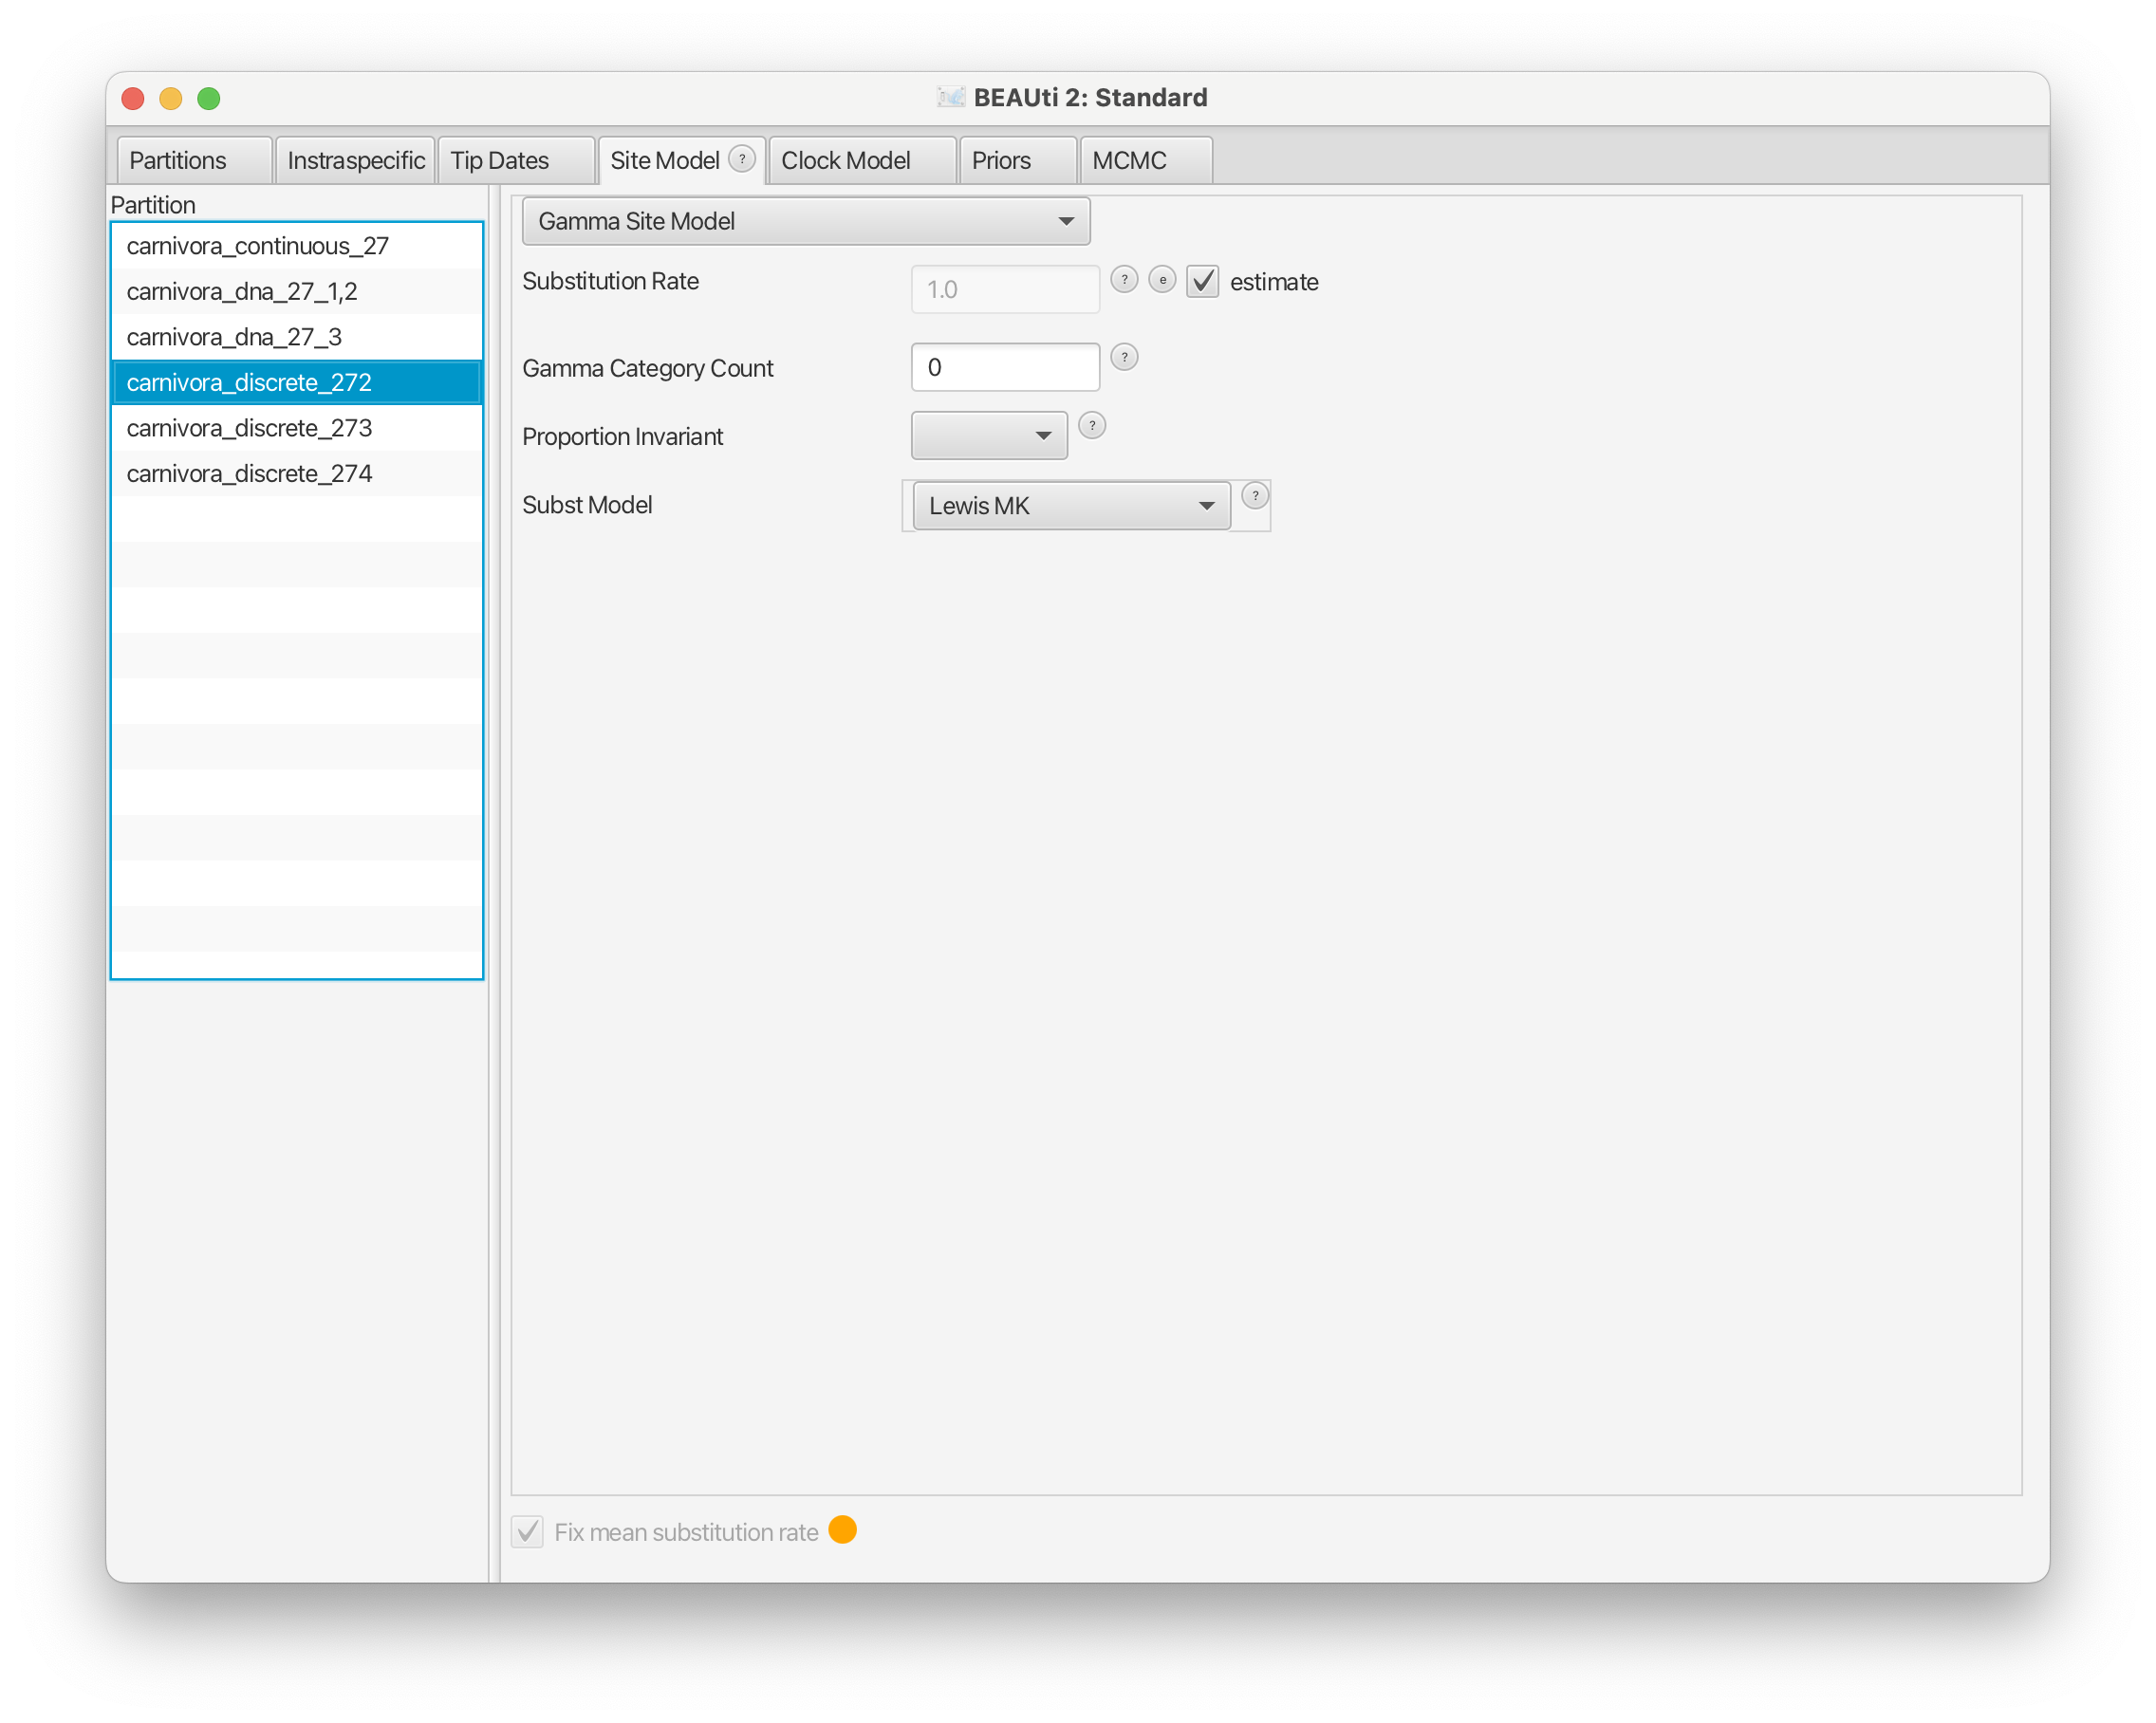
\includegraphics[width=0.700000\textwidth]{figures/SiteModelMk.png}
     \caption{Setting site models for discrete characters.}
    \label{fig:example11}
\end{figure}


\subsubsection{Setting the Clock model}
Similar to section~\ref{bm-clock-model}, we assume a relaxed clock model for each data partition. The specifications are shown in \autoref{fig:example12}.

\begin{figure}[!htbp]
    \centering
    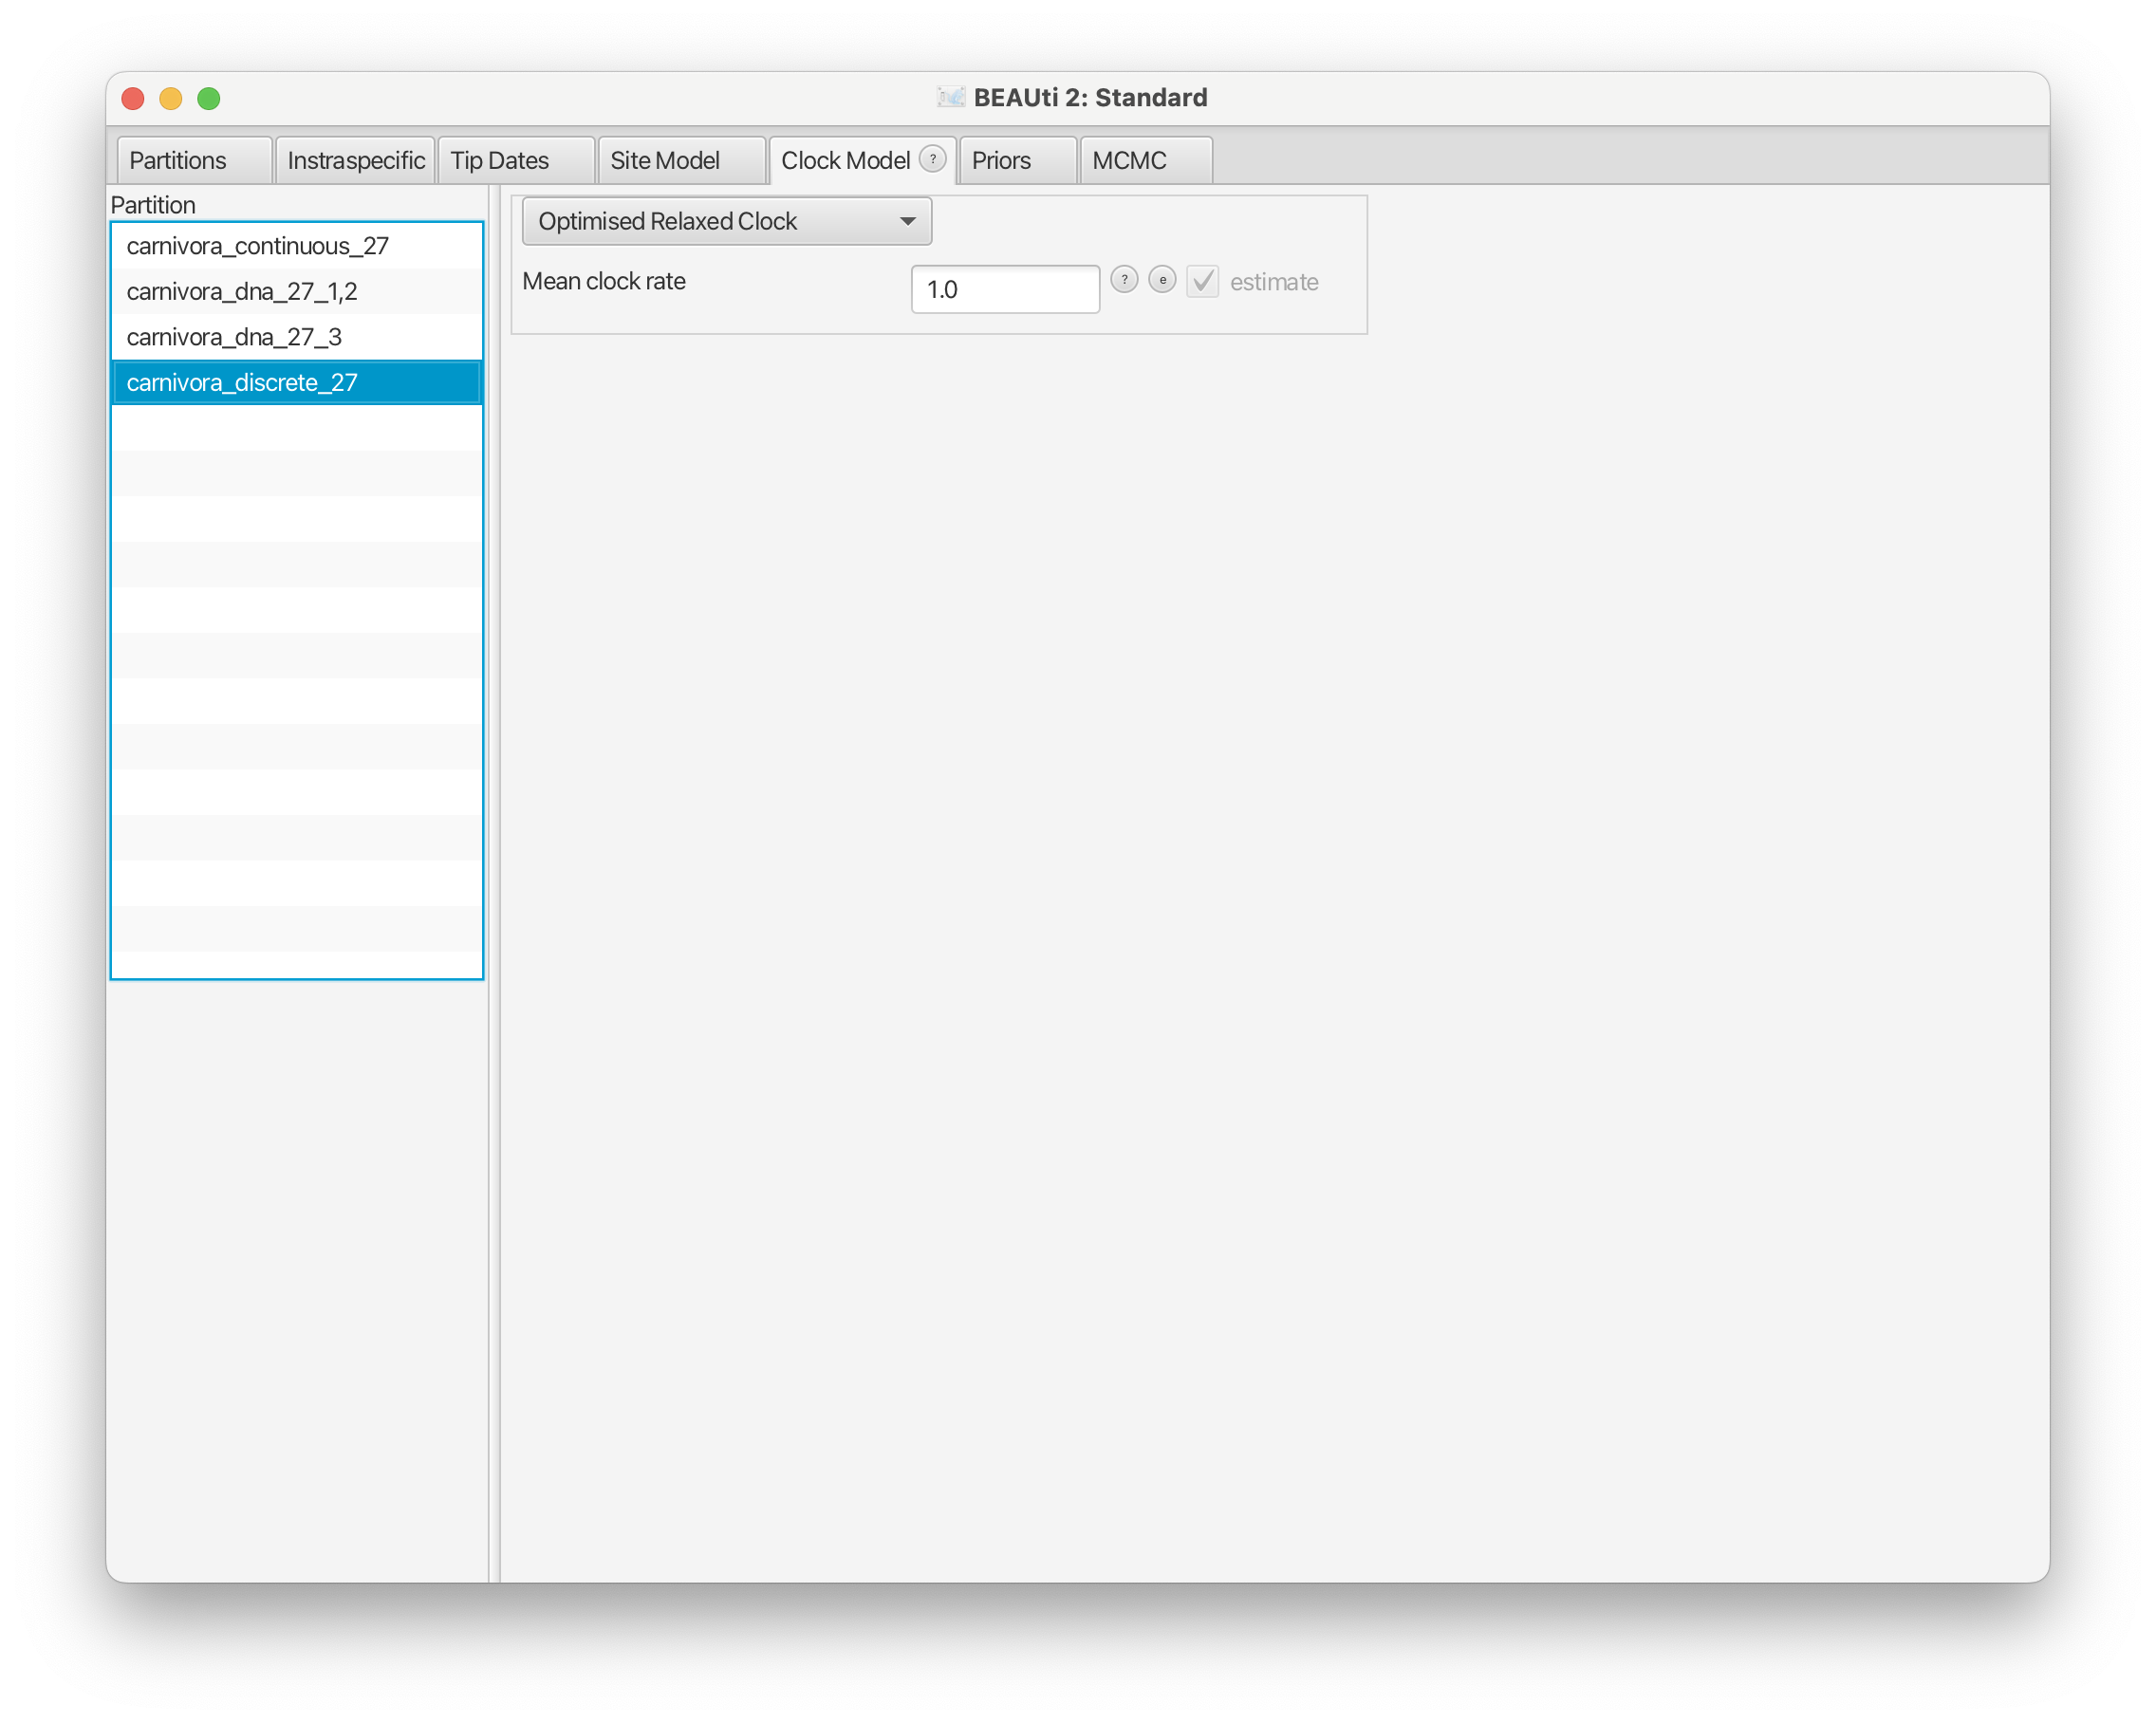
\includegraphics[width=0.700000\textwidth]{figures/ClockModel.png}
    \caption{Setting the clock models for continuous data, molecular data and discrete data.}
    \label{fig:example12}
\end{figure}

\subsubsection{Specifying the priors}

First, we select ''Fossilized Birth Death Model" from the drop-down menu and set it as the tree prior. Then we again retain the default priors for the rest of the parameters (\autoref{fig:example13}).

\begin{figure}[!htbp]
    \centering
    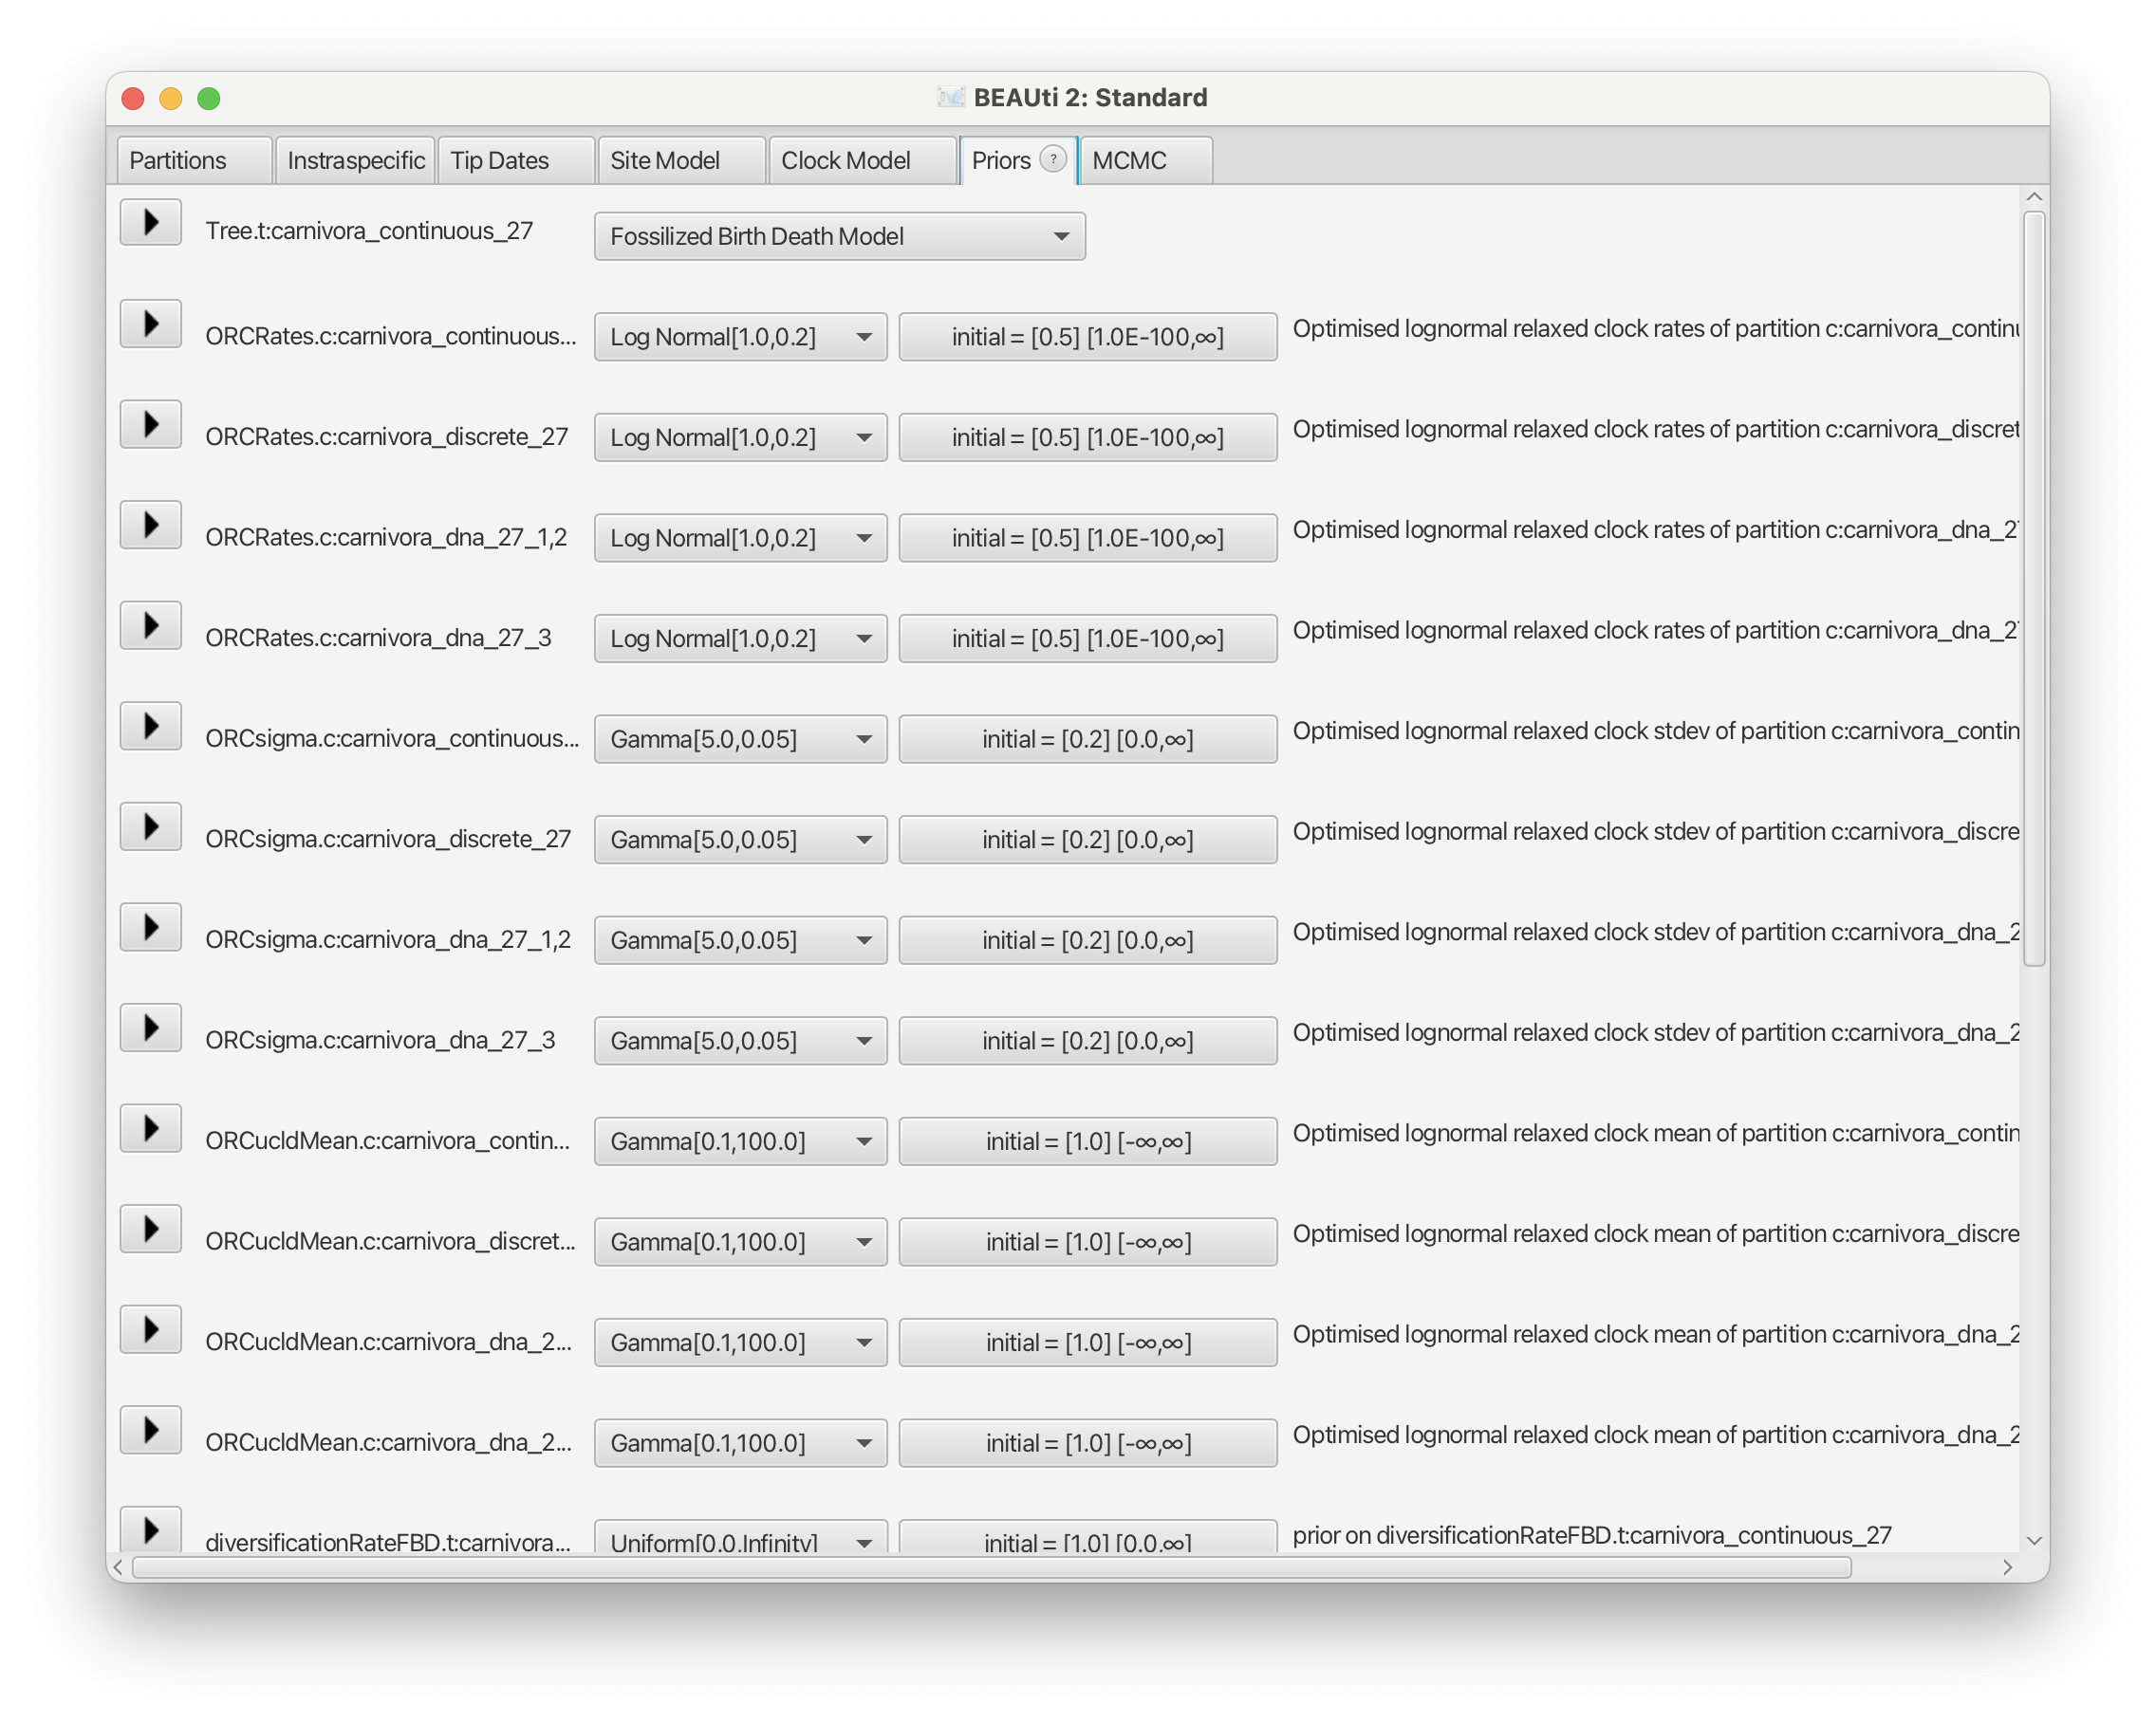
\includegraphics[width=0.700000\textwidth]{figures/Priors.png}
    \caption{Setting up tree model and  the prior distributions.}
    \label{fig:example13}
\end{figure}

\subsubsection{Specifying the MCMC chain length (MCMC)}\label{specify-the-mcmc-chain-length-mcmc}
%
Here we can set the length of the MCMC chain and after how many
iterations the parameter and trees a logged. For this dataset, 2 million
iterations should be sufficient. In order to have enough samples but not
create too large files, we can set the logEvery to 2000, so we have 1001
samples overall. Next, we have to save the \lstinline!*.xml! file under
\emph{File \textgreater{}\textgreater{} Save as}.

\subsection{Running the Analysis using BEAST2}\label{run-the-analysis-using-beast2}
%
Run the \lstinline!*.xml! using BEAST2 or use finished runs from the
\emph{precooked-runs} folder. The analysis should take about 6 to 7
minutes.
%

\subsection{Analysing the results}

For this section either use the output files from your own analysis or use finished runs from the
\emph{precooked-runs} folder. 

\begin{itemize}
\item Examine the posterior estimates for the inferred clock models for continuous data, discrete data and molecular sequences in Tracer (\autoref{fig:bm_res6} and \autoref{fig:bm_res7})
\begin{figure}[!htbp]
    \centering
    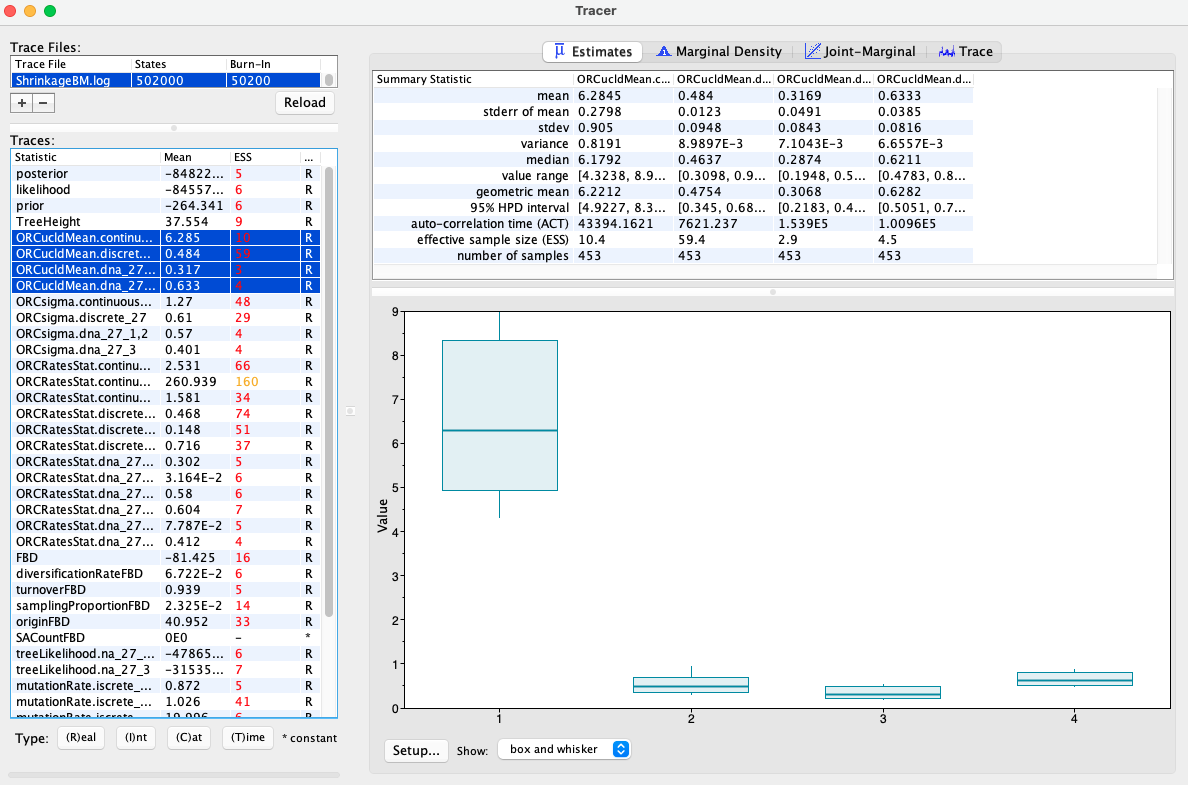
\includegraphics[width=0.700000\textwidth]{figures/results/EST_clock_rate.png}
    \caption{Estimated clock rates.}
    \label{fig:bm_res6}
\end{figure}

\begin{figure}[!htbp]
    \centering
    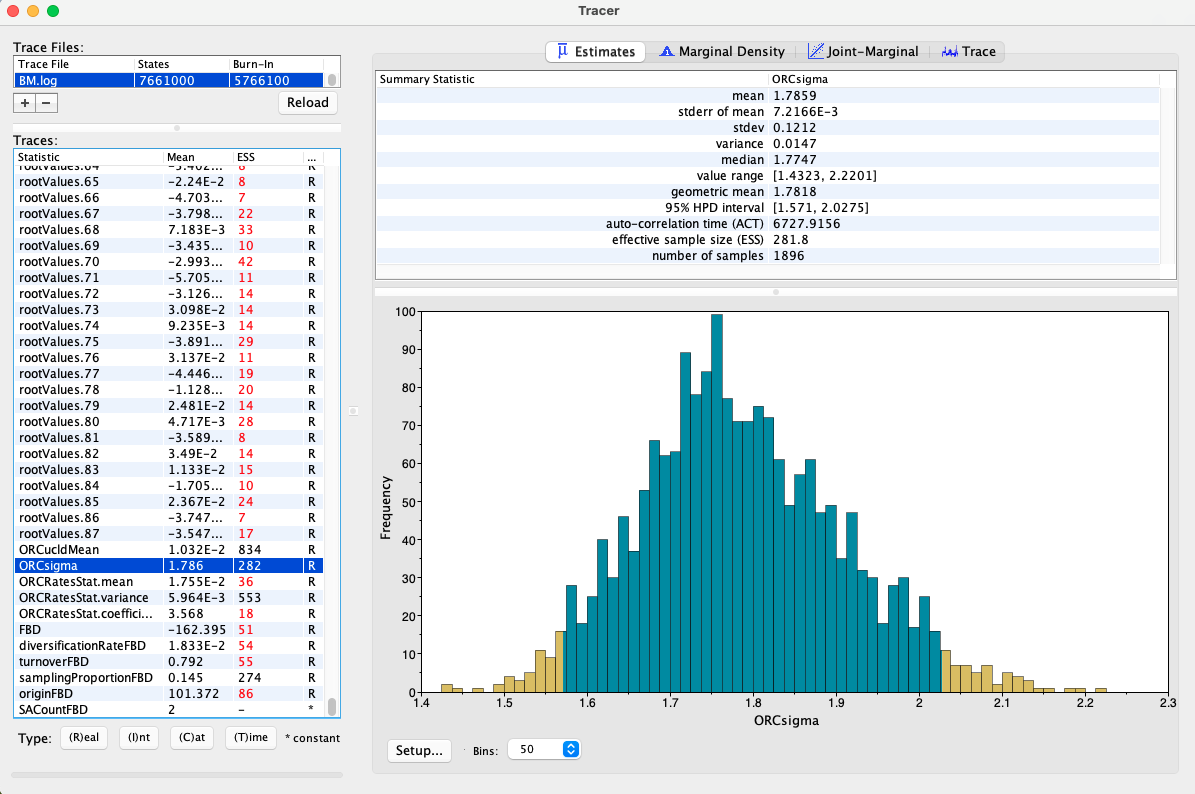
\includegraphics[width=0.700000\textwidth]{figures/results/BM_clock_sigma.png}
    \caption{Estimated standard deviations.}
    \label{fig:bm_res7}
\end{figure}

\item Construct the summary tree using TreeAnnotator (\autoref{fig:bm_res8})
\begin{figure}[!htbp]
    \centering
    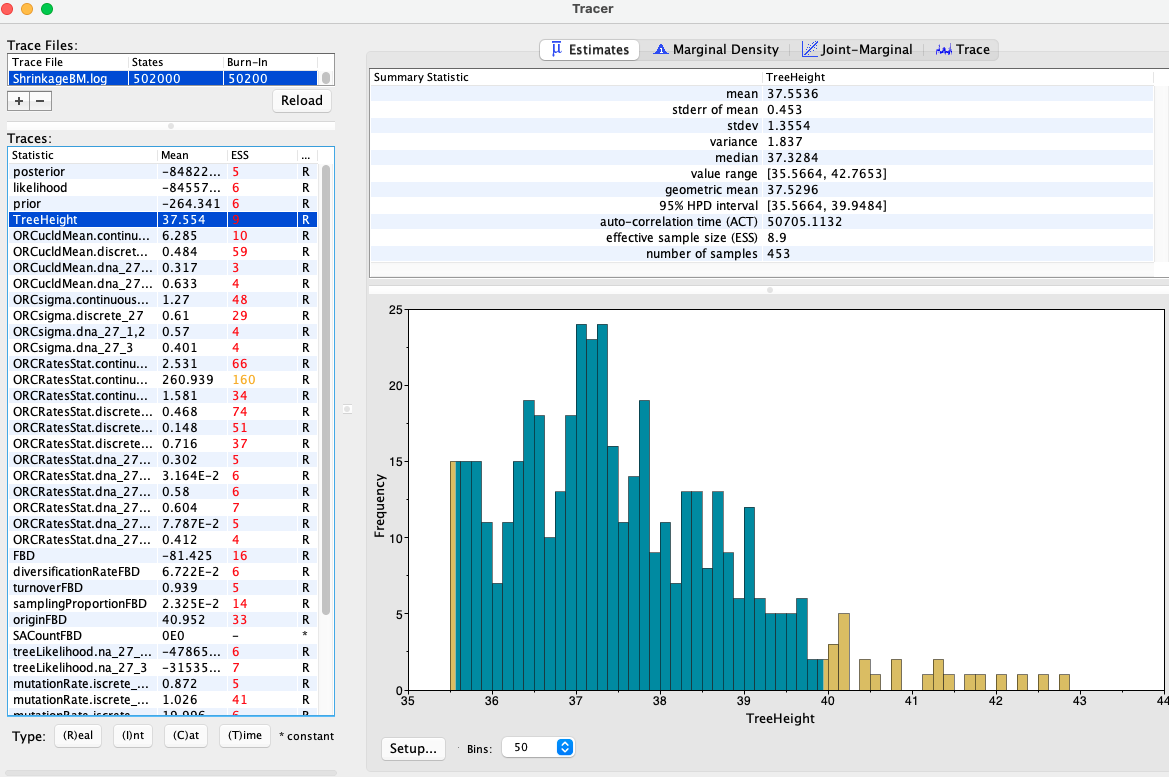
\includegraphics[width=0.700000\textwidth]{figures/results/EST_tree_height.png}
    \caption{Summarised MCC trees estimated from the combined data sets.}
     \label{fig:bm_res8}
\end{figure}
\end{itemize}


\section{Errors that can occur (Work in progress)}

One of the errors message that can occur regularly is the following:
\emph{Infinity likelihood}
% Not necessarily an error, could just be a very unlikely state, or more likely numerical underflow

\emph{Negative branch length}
% If this is in the MCC tree, this is not an error, just an unfortunate side effect of summarising a set of posterior trees into one tree. 

\emph{Unequal likelihoods}
% This seems serious and seems like a problem with the implementation of the BEAST2 package
\clearpage
%%%%%%%%%%%%%%%%%%%%%%%
% Tutorial disclaimer %
%%%%%%%%%%%%%%%%%%%%%%%
% Please do not change the license
% Add the author names and relevant links
% Add any other aknowledgments here
\href{http://creativecommons.org/licenses/by/4.0/}{
\includegraphics[scale=0.8]{figures/ccby.pdf}} This tutorial was written by Rong Zhang and F\'{a}bio K. Mendes for \href{https://taming-the-beast.github.io}{Taming the BEAST} and is licensed under a \href{http://creativecommons.org/licenses/by/4.0/}{Creative Commons Attribution 4.0 International License}. 

%%%%%%%%%%%%%%%%%%%%
% Do NOT edit this %
%%%%%%%%%%%%%%%%%%%%
Version dated: \today




%%%%%%%%%%%%%%%%
%  REFERENCES  %
%%%%%%%%%%%%%%%%

\printbibliography[heading=relevref]


\end{document} 